\documentclass[zihao=-4,a4paper]{ctexart}

%===================   导言区    ================================================================
% 加载字体相关宏包,支持设置英文字体和中文字体
\usepackage{fontspec}       % fontspec 宏包用于设置 OpenType 或 TrueType 字体,适用于 XeLaTeX 或 LuaLaTeX
\usepackage{xeCJK}          % xeCJK 宏包用于支持中文字体设置和排版

% 设置中文字体和主字体
\newcommand{\zhongsong}{\CJKfontspec{华文中宋}}  % 定义 \zhongsong 命令,使用华文中宋字体用于中文部分
\setmainfont{Times New Roman}                    % 设置主字体为 Times New Roman,适用于英文部分

% 数学相关
\usepackage{amsmath}    % AMS LaTeX 数学公式增强(align, cases, split 等)
\usepackage{amsthm}     % 定理环境(theorem, lemma, corollary)
\usepackage{amsfonts}   % 数学字体(\mathbb, \mathfrak)
\usepackage{mathrsfs}   % 额外的花体数学符号(\mathscr)
\usepackage{bm}         % 加粗数学符号(\bm)
\newtheorem{example}{例}              % 创建一个新的定理环境,命名为 "example",并设置标题为 "例"(整体编号)
\newtheorem{theorem}{定理}            % 创建一个新的定理环境,命名为 "theorem",并设置标题为 "定理"(按章节编号)
\newtheorem{definition}{定义}         % 创建一个新的定理环境,命名为 "definition",并设置标题为 "定义"
\newtheorem{axiom}{公理}              % 创建一个新的定理环境,命名为 "axiom",并设置标题为 "公理"
\newtheorem{property}{性质}           % 创建一个新的定理环境,命名为 "property",并设置标题为 "性质"
\newtheorem{proposition}{命题}        % 创建一个新的定理环境,命名为 "proposition",并设置标题为 "命题"
\newtheorem{lemma}{引理}              % 创建一个新的定理环境,命名为 "lemma",并设置标题为 "引理"
\newtheorem{corollary}{推论}          % 创建一个新的定理环境,命名为 "corollary",并设置标题为 "推论"
\newtheorem{remark}{注解}             % 创建一个新的定理环境,命名为 "remark",并设置标题为 "注解"
\newtheorem{condition}{条件}          % 创建一个新的定理环境,命名为 "condition",并设置标题为 "条件"
\newtheorem{conclusion}{结论}         % 创建一个新的定理环境,命名为 "conclusion",并设置标题为 "结论"
\newtheorem{assumption}{假设}         % 创建一个新的定理环境,命名为 "assumption",并设置标题为 "假设"

% 文字边框
\usepackage[style=1]{mdframed}   % 带边框的文字块

% 列表格式控制
\usepackage{enumitem}            % 自定义有序列表格式(如 (1)、(2)、(3))

% 参考文献格式
\usepackage{gbt7714}             % 配置 GB/T 7714(中国国家标准)参考文献格式

% 附录管理(自动编号附录,并在目录中显示)
\usepackage[toc,page]{appendix}

% 图表相关
\usepackage{booktabs}                % 三线表(上粗中细下粗)
\usepackage{diagbox}                 % 分类表头(对角线表头)
\usepackage{longtable}               % 长表格支持(允许表格跨页)
\usepackage{multirow}                % 加载 multirow 宏包,支持在表格中合并多行
\usepackage{float}                   % 控制图片浮动位置(H 选项可强制固定)
\usepackage{subfigure}               % 加载 subfigure 宏包,用于在同一行中插入多个子图
\usepackage{graphicx}                % 加载 graphicx 宏包,支持插入和缩放图像,常用于嵌入png、jpg等格式的图像
\usepackage{caption}                 % 加载 caption 宏包,用于自定义图表的标题和格式
\usepackage{color,xcolor}            % 加载 color 和 xcolor 宏包,支持文本、背景、框等内容的彩色设置
\captionsetup{labelsep=quad}         % 设置图形标题中标签和标题之间的分隔符为 "quad"(相当于一个空格宽度)
\renewcommand{\thesubfigure}{(\arabic{subfigure})}  % 重新定义子图编号的格式,使用圆括号括住阿拉伯数字编号

% 脚注等符号相关
\usepackage{pifont}                   % 提供 Dingbat 符号,包括带圈数字(①②③…)
\usepackage[symbol*,stable]{footmisc} % 增强脚注功能,支持符号脚注
\DefineFNsymbols{circled}{            %自定义带圈数字作为脚注符号
  {\ding{192}}  % ①
  {\ding{193}}  % ②
  {\ding{194}}  % ③
  {\ding{195}}  % ④
  {\ding{196}}  % ⑤
  {\ding{197}}  % ⑥
  {\ding{198}}  % ⑦
  {\ding{199}}  % ⑧
  {\ding{200}}  % ⑨
  {\ding{201}}  % ⑩
}
\setfnsymbol{circled}                 % 让脚注默认使用带圈数字
\usepackage{wasysym}                  % 提供额外的符号(例如圆圈符号、勾号等)

% 设置公式、表格和图形的编号规则,使其包含章节号
\numberwithin{equation}{section}  % 使公式编号以章节号为前缀(例如:1.1,2.3)
\numberwithin{table}{section}     % 使表格编号以章节号为前缀(例如:1.1,2.3)
\numberwithin{figure}{section}    % 使图形编号以章节号为前缀(例如:1.1,2.3)

% 页边距调整(提高排版美观)
\usepackage{geometry}
\geometry{top=2.5cm,bottom=2cm,left=2.5cm,right=2cm}

% 页眉页脚设置
\usepackage{fancyhdr}          % 加载 fancyhdr 宏包,用于自定义页眉和页脚
\pagestyle{fancy}              % 启用 fancyhdr 宏包的自定义样式
\fancyhf{}                     % 清空页眉和页脚的默认内容
\fancyhead[C]{\zihao{5}  \songti 武汉理工大学毕业设计} % 设置页眉内容:宋体5号居中
\fancyfoot[C]{~\zihao{5} \thepage~}                           % 设置页脚内容:页码居中
\renewcommand{\headrulewidth}{0.65pt}                         % 设置页眉下方的横线宽度为0.65pt

\usepackage{titlesec}
\setlength{\baselineskip}{20pt}  % 设置段落的行距为 20 磅

% 设置标题的段前、段后间距
\titlespacing{\chapter}{0pt}{0.5\baselineskip}{0.5\baselineskip}  % 章标题
\titlespacing{\section}{0pt}{0.5\baselineskip}{0.5\baselineskip}  % 节标题
\titlespacing{\subsection}{0pt}{0.6\baselineskip}{0.5\baselineskip}  % 小节标题

% 章节标题格式设置
\ctexset{
    section = {                                         % 章节标题设置
        format = \centering\bfseries\zihao{-2} \heiti,  % 章节标题居中,使用黑体小二号
        name = {第, 章}                                 % 章节标题格式为“第X章”
    },
    subsection = {                                      % 小节标题设置
        format = \bfseries\zihao{3} \heiti          % 小节标题使用黑体三号
    },
    subsubsection = {                                   % 子小节标题设置
        format = \bfseries\zihao{4} \heiti          % 子小节标题使用黑体四号
    }
}

% 链接相关
\usepackage{hyperref}     % 加载 hyperref 宏包,支持文档中的交叉引用和超链接(如点击跳转)
\hypersetup{              % 设置链接颜色为黑色
	colorlinks=true,
	linkcolor=black,
	filecolor=black,      
	urlcolor=black,
	citecolor=black,
}

% 源代码和绘图相关
\usepackage{listings}                % 加载 listings 宏包,用于在 LaTeX 文档中粘贴源代码并高亮显示
\usepackage{tikz}                    % 加载 tikz 宏包,提供强大的图形绘制功能
\usepackage{tikz-3dplot}             % 加载 tikz-3dplot 宏包,扩展 tikz 用于绘制三维图形
\usetikzlibrary{shapes,arrows,positioning} % 加载 tikz 库,提供绘制形状、箭头、定位等功能
\usepackage[ruled]{algorithm2e}      % 伪代码,支持 if-else、for 等结构

% 重新定义文档元素的名称
\renewcommand{\contentsname}{目 ~~ 录}      % 将目录部分的标题修改为 "目  录" 
\renewcommand{\abstractname}{摘 ~~ 要}      % 将摘要部分的标题修改为 "摘  要"
\renewcommand{\refname}{参考文献}           % 将参考文献部分的标题修改为 "参考文献"
\renewcommand{\indexname}{索引}             % 将索引部分的标题修改为 "索引"
\renewcommand{\figurename}{图}              % 将图形部分的标题修改为 "图"
\renewcommand{\tablename}{表}               % 将表格部分的标题修改为 "表"
\renewcommand{\appendixname}{附录}          % 将附录部分的标题修改为 "附录"
\renewcommand{\proofname}{证明}             % 将证明部分的标题修改为 "证明"
\renewcommand{\algorithmcfname}{算法}       % 将算法部分的标题修改为 "算法"
%===================   结束导言   ===============================================================


%===================   正文区    ================================================================
\begin{document}

%============== 封皮和前言 =================
%===============  封面  =================
\smallskip
\begin{center}

\vspace*{2.2cm}
\zhongsong{\zihao{1} 武汉理工大学毕业设计} \\
\vspace*{3.3cm}
\heiti{\zihao{2} 基于U-Net的医学图像语义分割方法研究}\\
\vspace*{5.5cm}

\zhongsong
\begin{tabular}{cc}
 \zihao{-2} 学院(系):&\underline{\makebox[7cm][c]{\zihao{-2}自动化学院}} \\ 
 \\
 \zihao{-2}专业班级: & \underline{\makebox[7cm][c]{\zihao{-2}自动化2105}} \\ 
 \\
 \zihao{-2}学生姓名: & \underline{\makebox[7cm][c]{\zihao{-2}李子豪}} \\ 
 \\
 \zihao{-2}指导教师: & \underline{\makebox[7cm][c]{\zihao{-2}赵希}} \\ 
 \\
\end{tabular} 
\end{center}
\thispagestyle{empty}

\pagestyle{empty}      % 封面页不显示页码
\cleardoublepage       % 确保新页码从右页开始(书籍排版)
\pagenumbering{Roman}  % 切换为罗马数字
\setcounter{page}{1}   % 强制页码从Ⅰ开始
\pagestyle{plain} 
\section*{\zihao{-2} \centering 摘 ~~ 要}

\vskip0.5cm

本文基于注意力机制提出了改进的U-Net模型AAH U-Net,通过在网络中嵌入注意力门,同时采用数据增强和混合损失函数策略,AAH U-Net最终实现了在多个医学图像数据集上的语义分割性能提升。

针对U-Net网络中跳跃连接会将大量来自编码器的背景噪声传递至解码器的问题,本文提出了改进的跳跃连接设计,通过在跳跃连接中嵌入注意力门模块动态地筛选并加权特征图,加强对编码器特征图的特征提取,从而提高模型对目标区域的定位能力。

针对单一损失函数难以适应医学图像中普遍存在的类别不平衡和边界模糊问题,AAH U-Net采用了混合函数策略,通过使用Dice损失函数和交叉熵损失函数的加权混合损失函数,兼顾模型在前景区域重叠度与像素级分类准确率的表现,整体提升模型的分割性能和训练稳定性。

针对医学图像分割任务中常见目标结构复杂且样本规模有限的场景,AAH U-Net模型使用了数据增强策略,通过对图像引入翻转、随机旋转等几何变换,增强模型对空间变换的鲁棒性和小样本学习能力。

凭借注意力门机制、数据增强和混合损失函数策略,AAH U-Net实现了在皮肤癌镜像数据集、肝癌CT数据集和脑部肿瘤MRI数据集上语义分割性能的大幅提升。相较于原U-Net网络,AAH U-Net在皮肤癌镜像数据集上的验证集Dice系数从0.75提升至0.83,相对提升约11\%,同时在肝癌CT数据集和脑部肿瘤MRI上的验证集Dice系数分别为0.89和0.83,均大幅优于U-Net模型。

所有代码和训练好的AAH U-Net模型已开源至github:\url{https://github.com/WBlackhole/Black_essay}。

{\zihao{4} \heiti 关键词:} \zihao{-4}U-Net\quad 医学图像语义分割\quad 注意力机制\quad 卷积神经网络\quad AAH U-Net

\vskip0.5cm

\addcontentsline{toc}{section}{摘要}

\clearpage
\section*{\zihao{-2} \centering \textbf{Abstract} }

This paper proposes an improved U-Net model, AAH U-Net, based on attention mechanisms. By embedding attention gates into the network and employing strategies such as data augmentation and hybrid loss functions, AAH U-Net achieves enhanced semantic segmentation performance across multiple medical image datasets.

To address the issue that skip connections in the original U-Net architecture tend to pass a large amount of background noise from the encoder to the decoder, this paper introduces an improved skip connection design. Attention gate modules are embedded within the skip paths to dynamically filter and weight feature maps, thereby enhancing the extraction of meaningful features from the encoder and improving the model's ability to localize target regions.

To tackle the difficulty of single loss functions in handling class imbalance and blurry boundaries common in medical images, AAH U-Net adopts a hybrid loss strategy. By combining the Dice loss and cross-entropy loss in a weighted manner, the model simultaneously improves foreground overlap accuracy and pixel-wise classification performance, leading to better segmentation results and training stability.

Considering the complex anatomical structures and limited sample sizes often encountered in medical image segmentation tasks, the AAH U-Net model incorporates data augmentation techniques such as flipping and random rotation. This enhances the model’s robustness to spatial transformations and improves its few-shot learning capability.

With the combined benefits of attention gates, data augmentation, and hybrid loss strategies, AAH U-Net achieves significant improvements in semantic segmentation performance on skin cancer dermoscopy datasets, liver cancer CT datasets, and brain tumor MRI datasets. Compared to the original U-Net, the Dice coefficient on the skin cancer dataset increased from 0.75 to 0.83 (a relative improvement of approximately 11\%), while the validation Dice scores on the liver CT and brain MRI datasets reached 0.89 and 0.83, respectively—both substantially outperforming the baseline.

All source code and pretrained models of AAH U-Net are publicly available at GitHub: \url{https://github.com/WBlackhole/Black_essay}.

\textbf{\zihao{4} Key Words:} U-Net\quad Medical Image Segmentation\quad Attention Mechanism\quad Convolutional Neural Network\quad AAH U-Net

\addcontentsline{toc}{section}{Abstract}
\pagestyle{empty}
\tableofcontents 
\thispagestyle{empty}

%============== 论文正文   =================
\pagestyle{fancy}
\pagenumbering{arabic}
\section{绪论}

\subsection{研究背景及意义}
\subsubsection{研究背景}

医学图像是指利用医学成像技术生成的视觉图像,涵盖计算机断层扫描(CT)、磁共振成像(MRI)、超声成像(US)等多种成像模态,通过分析其提供的组织结构、解剖细节及病理信息,放射科医师和内科医师可以快速准确地进行医疗诊断。对医学图像进行图像分割是分析的关键步骤之一,它涉及将图像划分为解剖结构或病灶区域(如器官、组织或病变)相对应的不同区域,这种支持肿瘤定位、器官边界划定的分割可以精确解释医学图像,为临床应用中的准确诊断、术前规划和定量分析奠定了基础\cite{panayides2020}。鉴于其重要性和对临床结果的直接影响,医学图像分割的准确性成为现代医疗健康系统工作中不可或缺的要求。然而,当前临床实践中大量依赖放射科医生手动标注分割图像,不仅耗时费力,还存在一定的主观性和一致性问题。尤其在高分辨率三维图像中,手动标注的工作量极大,容易引发标注者疲劳、遗漏或偏差,进而影响诊断质量。因此,伴随着医学图像数量的激增,研究高效、自动化且高精度的医学图像分割方法,不仅能偶减轻医生负担、提升标注一致性,更在促进智能辅助诊疗系统落地中扮演着不可替代的角色。

\begin{figure}[h]
    \centering
    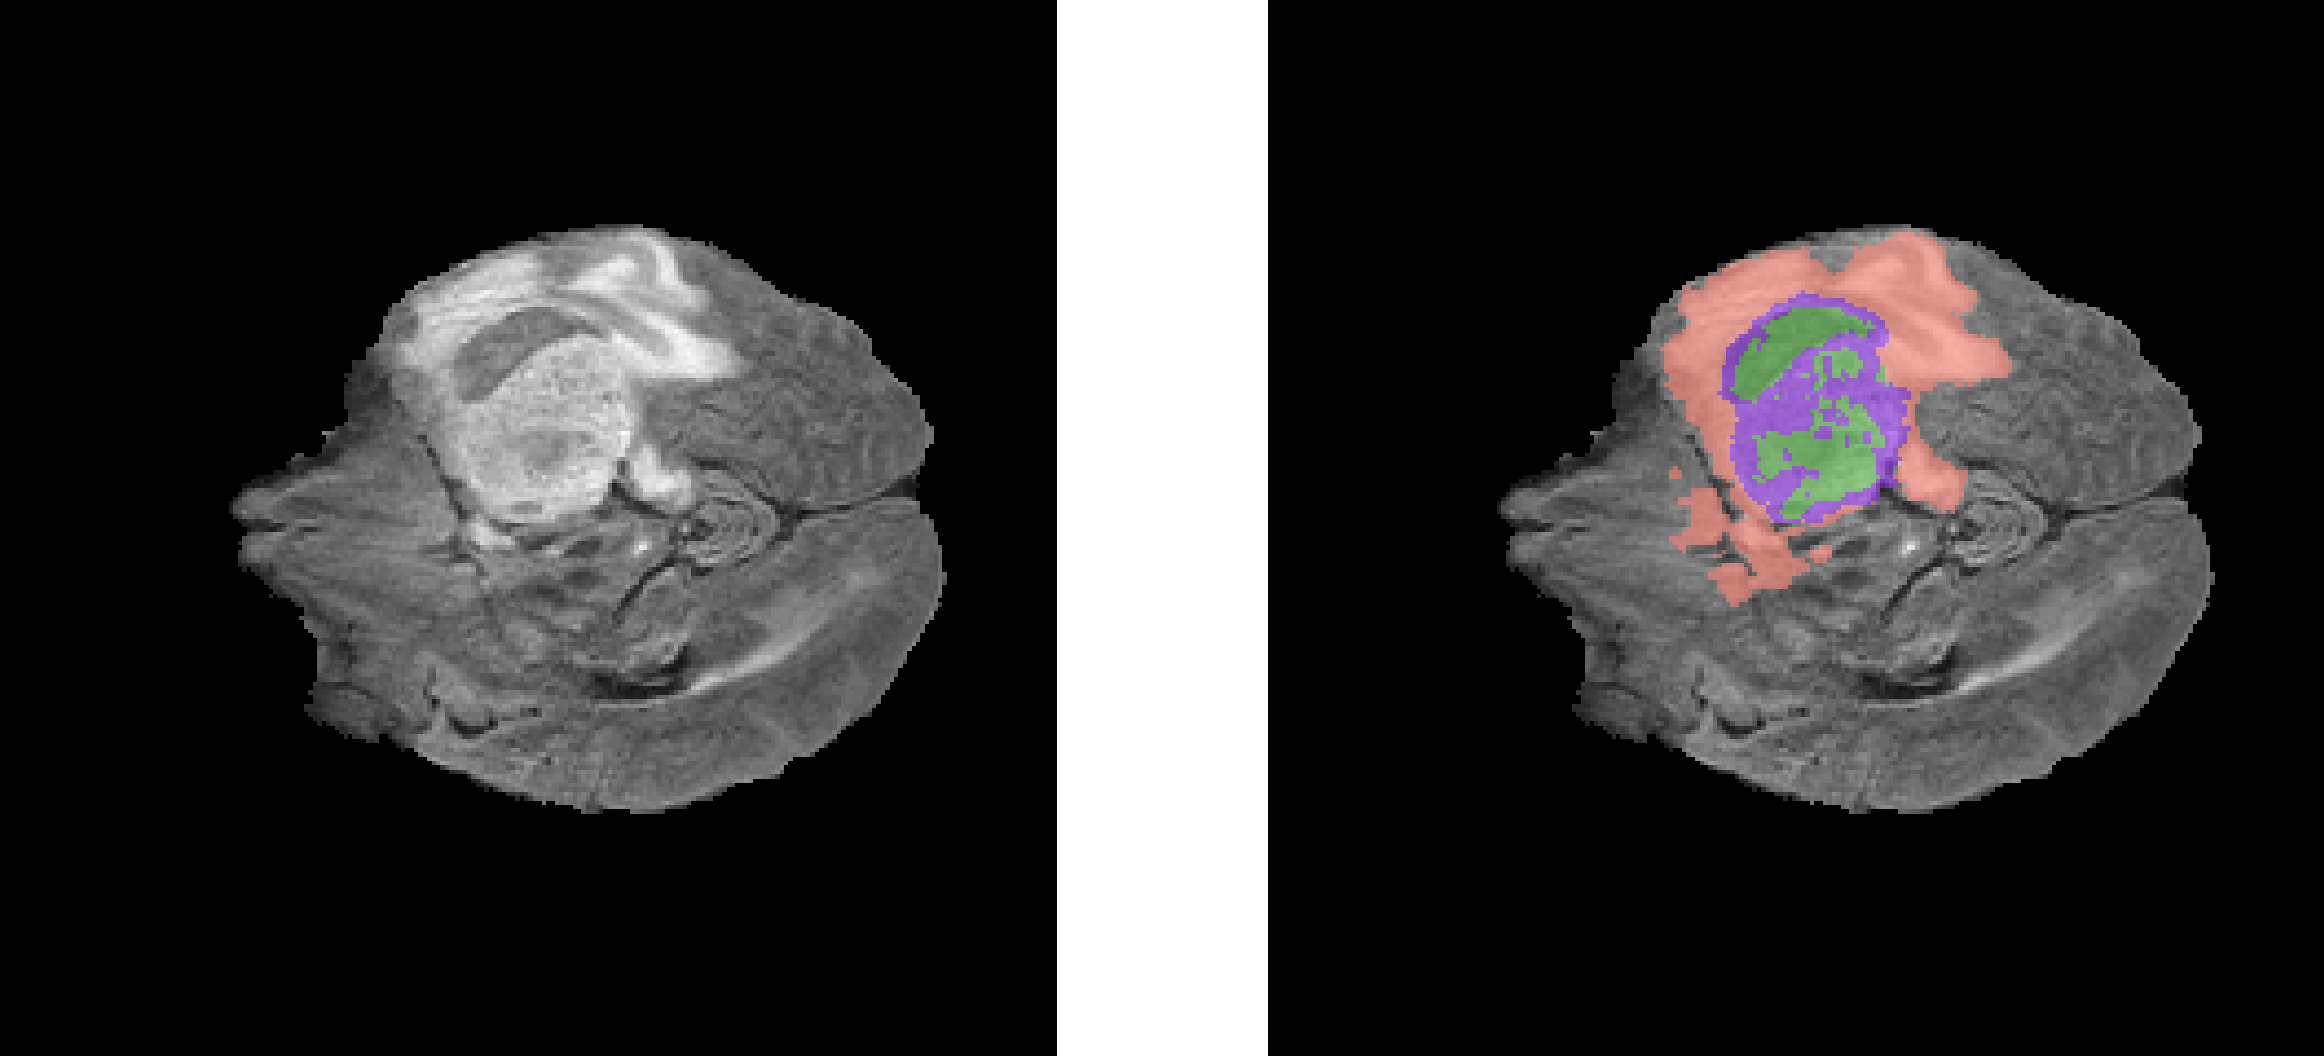
\includegraphics[width=0.77\textwidth]{fig/flair_and_mask.png}
    \caption{脑部MRI图像(左)及对应肿瘤手工标注结果(右)}
    \label{brian_tumor}
\end{figure}

在医学图像分割的发展早期,主要利用阈值分割、区域生长、边缘检测、聚类分割等传统算法进行组织、器官及病灶区域的识别与提取。这些方法大多依赖人工设计特征或强先验假设,基于像素灰度、边缘梯度、区域一致性等低层视觉信息构建规则,具有较高的可解释性和计算效率。然而,面对实际医学影像数据的复杂性,这些方法暴露出明显的局限性。医学影像中常见的解剖结构形态复杂、边界模糊(如肿瘤与周围组织过渡不清)、组织密度差异微弱,使得依赖简单灰度或梯度判断的传统方法难以准确建模区域间差异。此外,医学影像中的特殊挑战进一步削弱了传统方法的泛化能力与适应性:包括成像过程中引入的噪声干扰、患者间器官形态的个体差异与非线性形变、边界信息的不确定性、以及多模态成像之间强度分布的显著差异\cite{mohdsagheer2020}。这些因素对传统算法构成了严峻挑战,使其在跨患者、跨设备或跨模态应用中难以保持一致性能。同时,在临床实际应用中,常需依赖专业人员进行参数调整、种子点选择或后处理操作,操作流程繁琐、效率低下,严重制约了其在大规模医学影像分析系统中的推广与部署。基于上诉原因,尽管传统图像分割方法在特定条件下仍具参考价值,但其在面对复杂医学图像时的表达能力与适应性显然不足,亟需更具自动学习能力和结构建模能力的先进方法来突破其局限。

随着神经网络及深度学习的迅速发展和应用,以卷积神经网络为代表的深度学习方法在图像分类、检测与分割等计算机视觉任务中取得了突破性进展,其端到端的特征提取能力和强大的表征学习能力,使得图像分割任务由传统手工设计特征的范式,转向自动特征学习与高维特征建模的方向。而最早将深度学习应用于图像分割的代表性模型包括全卷积神经网络与SegNet等。全卷积神经网络通过去除全连接层,将图像映射为像素级别的类别预测图,是端到端分割网络的开端\cite{shelhamer2016};SegNet在其基础上引入池化索引进行上采样,提升了细节还原能力。至此,利用卷积神经网络等技术,深度学习方法凭借其优异的图像分割性能和适应性,在医学图像分割领域逐渐取代了传统算法的地位。然而,这些早期模型在医学图像场景下仍面临着一定局限:如对弱边界区域识别不敏感,对结构复杂或形变剧烈的解剖区域分割精度有限,且对小样本训练数据依赖较强,泛化能力不足等。

为应对医学图像小样本、边界模糊等挑战,Ronneberger等人\cite{ronneberger2015}于2015年提出了经典的U-Net模型,成为了医学图像分割领域的里程碑。U-Net采用编码器-解码器结构,前半部分通过卷积与池化提取高层语义特征,后半部分通过反卷积逐步还原空间分辨率。同时,网络在对称位置引入跳跃连接,将编码器中浅层的高分辨率特征与解码器中对应层的特征图进行拼接融合,从而有效弥补了深层语义特征中局部细节的丢失,实现了多尺度特征的整合与边界定位能力的增强。在ISBI细胞分割挑战赛中,U-Net凭借其出色的结构设计,以显著优势获得冠军。这一成功也推动了U-Net成为后续医学图像分割研究的基准模型,被广泛应用于脑肿瘤、乳腺癌、肺部病灶、眼底血管、皮肤病变等多种应用场景,并衍生出众多变体。U-Net的提出不仅标志着深度学习在医学图像分割领域的广泛应用起点,也为融合传统知识与深度模型提供了范式基础,奠定了现代医学图像分割算法的主流框架。

\begin{figure}[h]
    \centering
    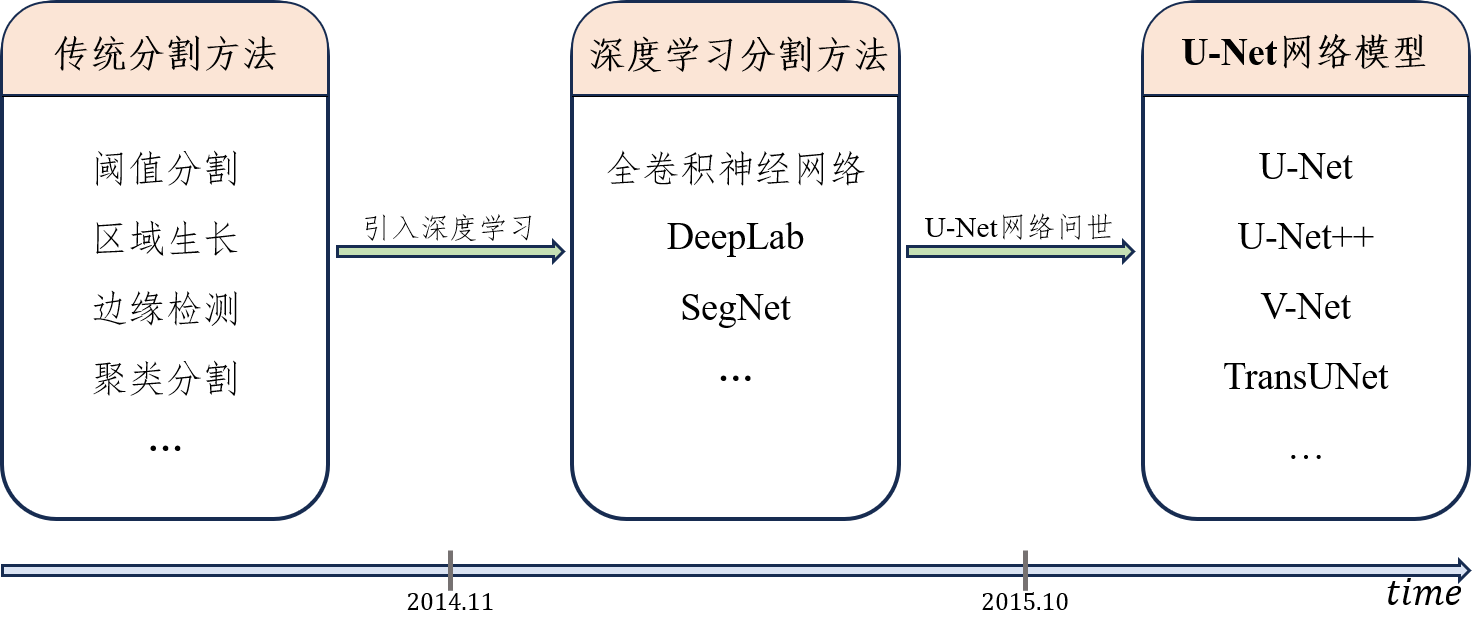
\includegraphics[width=\textwidth]{fig/develepment_of_seg.png}
    \caption{医学图像分割方法发展脉络}
    \label{develop_seg}
\end{figure}

尽管U-Net在医学图像分割中取得了巨大的成功,但随着临床场景的复杂化与精度需求的提高,原始U-Net在多种实际应用中仍存在显著局限性。首先,在多目标重叠、边界模糊或形态不规则的复杂场景中,U-Net的分割准确性容易下降。例如,面对多个病灶区域相互接近或重叠(如多发性肿瘤、血管交叉结构)时,模型难以有效区分各目标,易发生融合或漏检现象;对于尺寸较小的病灶(如早期病变、微小转移灶),因其在特征图中易被下采样过程压缩甚至丢失,导致分割结果中频繁出现漏检;此外,U-Net对输入图像质量也较为敏感,在存在伪影、噪声或成像伪差等干扰时,模型的鲁棒性难以保证\cite{azad2024}。

随着医疗影像技术的不断发展和临床需求的日益提升,医学图像分割任务面临着更高层次的挑战与期望。传统的二维静态图像处理已难以满足当前复杂的医学场景,特别是在涉及动态器官(如心脏、肺部)或介入手术导航等实时性强的应用中,分割模型不仅需要具备快速响应能力,还要在保持精度的同时实现高效率推理。此外,随着三维成像技术的普及,诸如CT、MRI等医学影像数据普遍具有体积属性,甚至在某些应用中演化为四维(随时间变化的3D序列)数据,这对模型提出了在空间与时间维度上同时建模的能力要求。因此,支持3D/4D数据结构处理已成为医学图像分割发展的重要方向。

针对上述高阶需求,现有研究虽已在多个方向取得一定进展,但仍存在明显空白,特别是如何针对具体医学应用场景对U-Net进行定制化改进的问题仍缺乏系统探索\cite{krithikaaliasanbudevi2022}。例如,对于多模态影像(如PET-CT、T1/T2-weighted MRI等)带来的信息互补特性,如何在U-Net结构中引入多模态融合机制,以提升模型对异构数据间语义关联的建模能力。此外,在实际临床环境中,分割模型常需部署于移动端、边缘设备或术中设备中运行,受限于算力、内存及功耗等资源约束,因此U-Net结构的轻量化设计亦成为关键研究方向之一,如采用深度可分离卷积、网络剪枝、知识蒸馏等手段减小模型体积和计算量,而不显著损失精度。总体而言,如何在保持U-Net核心优势的基础上,围绕注意力建模、多源信息融合与计算效率优化等维度进行针对性设计,构建适用于多样医学场景的高效、稳健、可解释的新型分割模型,是当前研究中亟需填补的重要空白。

\subsubsection{研究意义}

本研究的学术意义主要体现在三个方面:

从理论价值层面出发,对U-Net模型进行系统性改进,提升其对复杂结构、细粒目标及低对比度区域的建模能力,不仅有助于解决医学图像分割中的多个核心难题,也为设计具备更强表达能力与泛化能力的深度模型提供新的思路。而改进后的模型架构及训练策略在结构设计、信息流建模及优化方法等方面均具有一定的创新性,对医学图像语义分割任务的理论体系形成补充,也为应对小样本条件下的训练、提升模型鲁棒性及解释性等问题提供了具有借鉴价值的解法。

从应用价值层面出发,在实际临床中,医学图像分割是许多关键诊疗环节的基础,尤其在肿瘤检测、器官分割、病灶定量评估等任务中具有核心地位。提高分割模型的精度与效率,可有效辅助医生快速准确地定位病灶区域(如脑肿瘤、乳腺结节、血管斑块等),减少漏诊误判,提升诊断一致性,显著缓解医生的工作负担。特别是在多目标重叠、边界模糊等复杂场景中,基于改进U-Net的高性能模型可为医生提供更清晰、准确的辅助分割结果,提升临床诊疗的整体质量。同时,高质量的自动分割模型可广泛应用于放射治疗中的靶区勾画、术前路径规划、术中导航与术后评估中,减少对经验丰富医生的高度依赖,降低因人工勾画不一致带来的手术误差与放疗剂量偏差,为治疗过程的标准化与精细化提供技术保障。此外,结合患者的个体影像特征与多模态医疗数据,本研究成果也将为实现个性化医疗提供支持,如用于移植器官体积与形状评估、疗效追踪、慢病进展预测等,有助于推动以患者为中心的精准医疗落地。

从社会价值层面出发,根据WHO《世界健康统计2025》报告\cite{who2021stats},2023年全球医疗人员缺口高达1470万人,预计2030年仍将维持在1110万人以上,尤其是在非洲与东地中海占据近七成。这一结构性短缺为医学图像自动化分割等智能化辅助技术在全球范围内的应用提供了迫切现实背景,面向基层医疗或资源匮乏地区,轻量化、高精度、可部署性的医学图像分割模型可构建低成本的智能辅助诊断系统,缓解医资不均、专家短缺等公共卫生难题,推动普惠医疗的发展。因此,本研究不仅具备显著的学术理论价值,也具有广泛而深远的临床实践与社会应用前景。


\subsection{国内外研究现状}

自2015年Ronneberger等人提出U-Net以来,被引用超过73600次,其凭借高效的特征提取与恢复能力,在医学影像的任务中取得了广泛的应用,成为了医学图像分割领域最广泛使用的架构之一。然而,传统U-Net仍然存在显著的局限性:在全局信息建模和边界细化方面不足;感受野有限,难以捕捉全局上下文,对结构复杂或背景噪声大的区域理解不足;模型冗余大,计算成本高等。因此,近年来国内外学者针对这些问题以及不同的应用场景,在原始U-Net网络的基础上,通过优化结构、引入注意力机制、融合多尺度特征等方法,提出了多种改进模型。这些改进已在多篇相关综述类文章中被系统总结\cite{azad2024,krithikaaliasanbudevi2022,wang2023},下文中将根据Azad等人提出的U-Net变体分类法\cite{azad2024},对国内外学者的研究现状进行概述。

\subsubsection{国外研究现状}

当前国际学术界在医学图像分割领域主要围绕U-Net架构的改进与创新展开研究,重点研究方向包括:多尺度特征融合优化、混合架构创新和多模态处理突破。

多尺度特征融合策略可以通过组合来自不同空间分辨率或感受野范围的特征,增强网络对不同大小、模糊边界目标的识别能力。因此,许多改进模型通过改进U-Net网络的跳跃连接以增强U-Net网络的多尺度特征融合,以提高其上下文建模能力。Zhou等人\cite{zhou2018}提出了Unet++模型,通过密集跳跃连接优化特征重用,相较于U-Net网络只融合同层级的编码器和解码器特征图,UNet++实现了更精细的多尺度特征融合,改善了小目标与弱边界的分割性能。OKtay等人\cite{oktay2018}最早将注意力机制引入U-Net,通过在跳跃连接中引入注意力门(Attention Gates, AGs),他们提出了attention U-Net模型。attention U-Net可以根据高层语义信息和浅层特征图联合计算注意力权重,增强对目标区域的响应抑制无关区域的响应,同时避免冗余的模型结构。通过在跳跃连接中引入双向卷积LSTM(long-term-short-term-memory)模块,Azad等人\cite{azad2019}提出了BCDU-Net模型,将来自编码器和解码器的特征图在双向卷积LSTM中进行组合,提供了丰富的同时包含语义和局部信息的特征图。

在对称的编码-解码器结构中,通过编码器提取多层次语义特征并压缩空间信息,解码器逐步恢复分辨率并融合浅层细节,可以实现对目标区域的精准分割。相较于U-Net采用卷积神经网络作为编码-解码结构层,许多研究者通过采用或结合不同的网络层来构建U-Net,以提高网络的语义分割能力。受残差网络的启发,Drozdzal等人\cite{drozdzal2016}提出了residual U-Net网络,包含编码-解码层的长跳跃连接和卷积网络层之间跨层的短跳跃连接,实现了相较于原始U-Net网络更快的训练收敛。同样的,Milletari等人\cite{milletari2016}提出了采用3D残差块作为网络主体的V-Net模型,能够实现对3D图像更快更精确的分割。Ibtehaz等人\cite{ibtehaz2020}提出的MultiResUnet则基于Inception块,通过并行堆叠3×3、5×5和7×7卷积核捕获多尺度特征,在保持参数效率的同时,显著提升了模型对多尺寸目标的适应性。此外,Karaali等人\cite{karaali2022}利用密集残差块提出了Residual Dense-Net(RDN),使得特征在局部密集连接中传播的同时,也具备跨单元的残差路径,提升了模型表达能力和训练稳定性。

% 补充例子
位于编码器和解码器中间最底层的瓶颈区域(Bottleneck)代表了输入数据最深层的语义,其分辨率最低通道数最多,对整体性能影响极大。因此,许多研究通过增强瓶颈区域来提升模型对复杂结构的建模能力,弥补压缩造成的信息损失。其中,许多研究者选择引入注意力机制。例如,Guo等人\cite{guo2021}通过在Bottleneck区域引入空间注意力模块(Spatial Attention Module)提出了SA-UNet模型,其设计兼顾性能提升和计算效率,尤其适合处理低信噪比、高结构复杂性的医学图像。

近年来,Transformer模型在自然语言处理(Natural Language Processing, NLP)中表现优异,受此启发,不少研究者将Transformer模型引入至视觉识别任务中。Chen等人\cite{chen2021}在U-Net网络的编码器中引入ViT(Viision Transformer)模型,通过图像化嵌入提取全局上下文谢谢,同时保留卷积神经网络增强局部特征,一定程度上弥补了U-Net对长距离依赖建模能力的不足。Azad等人\cite{azad2022}则利用ViT的全局信息增强的特点,提出了contextual attention network(TMU)模型,通过自适应地融合U-Net生成的局部特征与ViT的全局信息,增强医学图像中重叠边界区域的分割效果。

为了获得丰富的特征表示,医学图像分割领域常用的方法是多尺度与多模态方法。其核心目标在于通过综合利用多模态或多尺度图像中的全部可用信息,同时保留最理想且相关的特征,从而提升训练模型的性能。Dolz\cite{dolz2018}等学者在Dense Multi-path U-Net中提出的创新架构,通过模态融合和Inception模块扩展两方面增强了传统U-Net的丰富表征学习能力,解决了传统多模态分割中早期和晚期融合无法充分建模模态间复杂关系的问题。除此之外,Lachinov等人\cite{lachinov2019}提出的Cascaded Unet通过并行多编码器架构,实现了多模态MRI数据的模态特异性特征提取,克服了原始U-Net对多模态数据同质化处理的局限性。

\begin{table}[!htbp]
  \centering
  \caption{U-Net变体模型的国外改进策略对比}
  \label{tab:unet_var_en}
  \small
  \begin{tabularx}{\textwidth}{@{}C C C@{}}
    \toprule
    \textbf{U-Net变体类别}  
      & \textbf{模型名称} 
      & \textbf{核心改进} \\ 
    \midrule
    \multirow{3}{*}{跳跃连接改进} 
      & UNet++ & 密集跳跃连接跨层级特征融合 \\ \cmidrule(lr){2-3}
      & Attention U-Net & 跳跃连接中嵌入注意力门 \\ \cmidrule(lr){2-3}
      & BCDU-Net & 双向卷积LSTM模块特征融合 \\
    \midrule
    \multirow{4}{*}{主干网络改进} 
      & Residual U-Net & 采用残差块进行长短跳跃连接 \\ \cmidrule(lr){2-3}
      & V-Net & 采用3D残差块处理3D数据 \\ \cmidrule(lr){2-3}
      & MultiResUnet & 采用多尺度并行卷积核 \\ \cmidrule(lr){2-3}
      & RDN & 采用密集残差跨单元路径 \\  
    \midrule
    \multirow{2}{*}{混合Transformer架构} 
      & TransUNet	& 编码器引入ViT提取全局信息 \\ \cmidrule(lr){2-3}
      & TMU & 融合ViT与U-Net特征增强边界 \\
    \midrule
    \multirow{2}{*}{多层次特征增强}
      & Dense Multi-path U-Ne & 多模态融合结合Inception结构 \\ \cmidrule(lr){2-3}
      & Cascaded U-Net & 并行多编码器提取模态特征 \\
    \bottomrule
  \end{tabularx}
\end{table}

综上所述,可以发现,国外医学图像分割研究在算法的创新性、数据资源丰富度及跨学科合作的紧密性等方面表现出明显优势。研究者尝试将Transformer、注意力机制、多模态融合等最新技术融入UNet结构中,不断突破传统模型的局限。但是,国外研究在某些复杂场景下仍存在明显不足,例如对多器官重叠、小病灶等困难场景的分割仍具挑战性,且现有模型在临床应用中的可解释性不足,难以清晰展示决策依据,这成为未来医学图像分割领域的重要发展方向。总体而言,国外的研究持续深入地推动着医学图像分割领域的发展,不断丰富方法论与实践经验,为医学人工智能的发展奠定了坚实基础。

\subsubsection{国内研究现状}

近些年,国内研究者紧跟国际研究的步伐,积极探索U-Net模型改进与应用落地,提出了大量的创新模型及改进方法,主要围绕多尺度特征融合、混合架构设计和轻量化应用三大方向展开创新,兼具理论突破与实际价值。

在U-Net++模型的基础上,Huang等人\cite{huang2020}提出了U-Net3+模型,通过全尺度跳跃连接实现全尺度特征融合显著提高了小目标和模糊边界的识别精度。而Li等人\cite{li2020}提出的Attention U-Net++模型则在U-Net++模型的所有跳跃连接中引入注意力机制,从而动态筛选重要特征区域,抑制无关噪声。此外,Xiang等人\cite{xiang2020}则创新性的提出了双向O型网络(BiO-Net),通过引入双向跳跃连接机制将解码器的高层语义特征反馈回同层编码器,形成闭环信息流,使得编码器能够利用解码器的全局上下文,提升对复杂结构的建模能力。

侯向丹等人\cite{HouXiangDan2023}提出的TCU-Net在保持U—Net编解码整体框架的基础上,进行了双重增强设计,融合ResNet和Transformer构建混合感受野,可用有效结合局部细节与全局上下文信息,大幅提升对血管等细小组织的感知能力。

Wang W等人\cite{wang2021}结合3D CNN作为编码器,Transformer模块作为瓶颈捕捉局部-全局信息,这种设计增强了MRI等跨切片数据的语义建模能力。此外,Li等人\cite{li2021}将Group Transformer插入U-Net各层,通过交替卷积与多头自注意模块提高感受野,同时通过引入Fourier描述子孙是,提示边界模糊区域的分割能力。也有研究者彻底舍弃卷积神经网络作为编码器与解码器的主干模块,Cao等人\cite{cao2021}采用Swin Transformer作为U-Net网络的主干结构,搭配滑动窗口注意力,构建了纯Transformer网络,提升全局上下文捕捉能力。

\begin{table}[!htbp]
  \centering
  \caption{U-Net变体模型的国内改进策略对比}
  \label{tab:unet_var_ch}
  \small
  \begin{tabularx}{\textwidth}{@{}C C C@{}}
    \toprule
    \textbf{U-Net变体类别}  
      & \textbf{模型名称} 
      & \textbf{核心改进} \\ 
    \midrule
    \multirow{3}{*}{跳跃连接改进} 
      & U-Net3+ & 全尺度跳跃融合细粒特征 \\ \cmidrule(lr){2-3}
      & Attention U-Net++ & 密集跳跃连接引入注意力筛选 \\ \cmidrule(lr){2-3}
      & BiO-Net & 双向跳跃闭环语义反馈\\
    \midrule
    \multirow{4}{*}{混合Transformer} 
      & TCU-Net & 采用残差块和Transformer双增强 \\ \cmidrule(lr){2-3}
      &  & 采用3D残差块处理3D数据 \\ \cmidrule(lr){2-3}
      & Group Trans-U-Net & 交替卷积与Group注意融合 \\ \cmidrule(lr){2-3}
      & Swin-Unet & Swin Transformer替代卷积主干 \\  
    \midrule
    \multirow{2}{*}{轻量化设计} 
      & MRUNet	& 两阶段协同进行轻量分割检测 \\ \cmidrule(lr){2-3}
      & TinyU-Net & 级联感受野提升轻量表达力 \\
    \bottomrule
  \end{tabularx}
\end{table}

Wang F等人\cite{Wang2023T}借鉴Mask R-CNN的思路提出了MRUNet模型,通过两阶段检测-分割协同和轻量化设计,显著提升了复杂农业场景下昆虫幼虫识别的准确率与稳定性,为农业AI应用提高了可靠解决方案。Chen等人\cite{chen2024}提出的TinyU-Net轻量化模型,专为资源受限环境下的医学图像自动分割任务而设计,通过一种级联的感受野扩展策略,在不同的通道间挖掘冗余信息,增强特征表达能力,同时有效控制计算成本和参数规模。

综上所述,国内的研究已从理论跟跑逐步转向应用领跑,未来需在基础模型创新和垂直场景深耕间持续协同,推动技术向产业端的规模化落地。

\subsection{研究内容与创新点}
%明确本论文的研究内容,包括对U - Net网络结构的分析、改进方法的探索以及实验验证等。
%突出本研究的创新点,如对网络结构的优化、新数据增强方法的引入等。


\subsection{论文组织结构}
%简要介绍各章节的主要内容和逻辑关系。

\section{相关技术与理论基础}

\subsection{医学图像语义分割基础}

图像分割任务可以分为两个不同的任务类别:语义分割任务和实例分割任务\cite{azad2024}。语义分割是像素级图像分割,图像中的每个像素点都有一个对应的类别,语义分割任务则需要尽量正确预测每个像素点的类别。如图~\ref{fig:seg}所示,实例分割在语义分割任务的基础上,需要将同类别的像素分类为不同的对象实例,即同类不同例。基于医学图像的语义分割任务则是指利用计算机视觉技术去分析和处理2D或3D医学图像,达到将人体器官、软组织和病灶体进行分割、提取,三维重构和展示的目的\cite{liu2021}。

\begin{figure}[htbp]
    \centering
    \subfloat[原图]
    {
        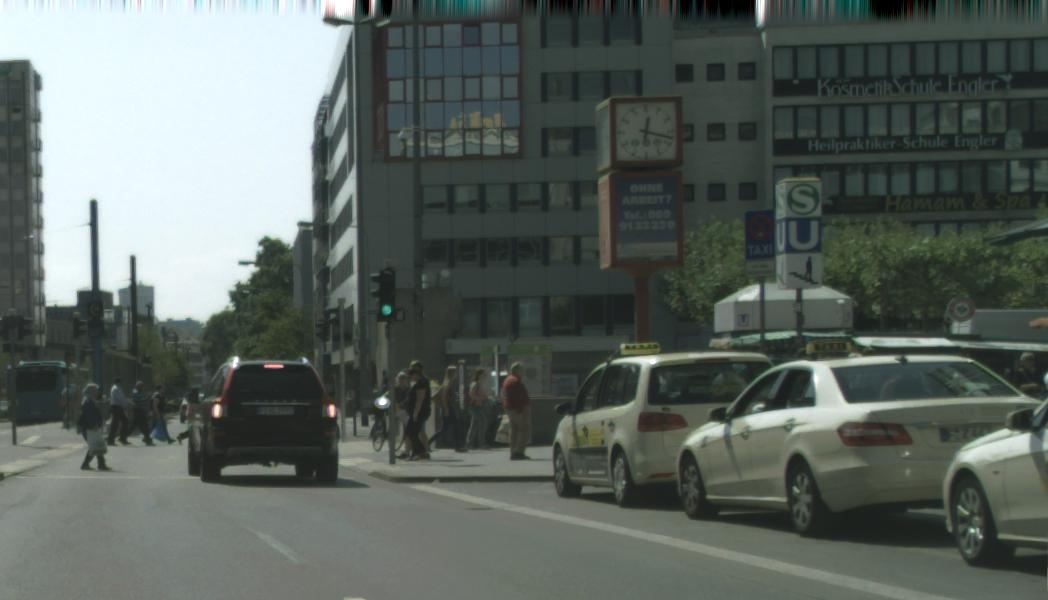
\includegraphics[width=0.3\textwidth]{fig/img_seg.jpg}
    }
    \subfloat[语义分割图]
    {
        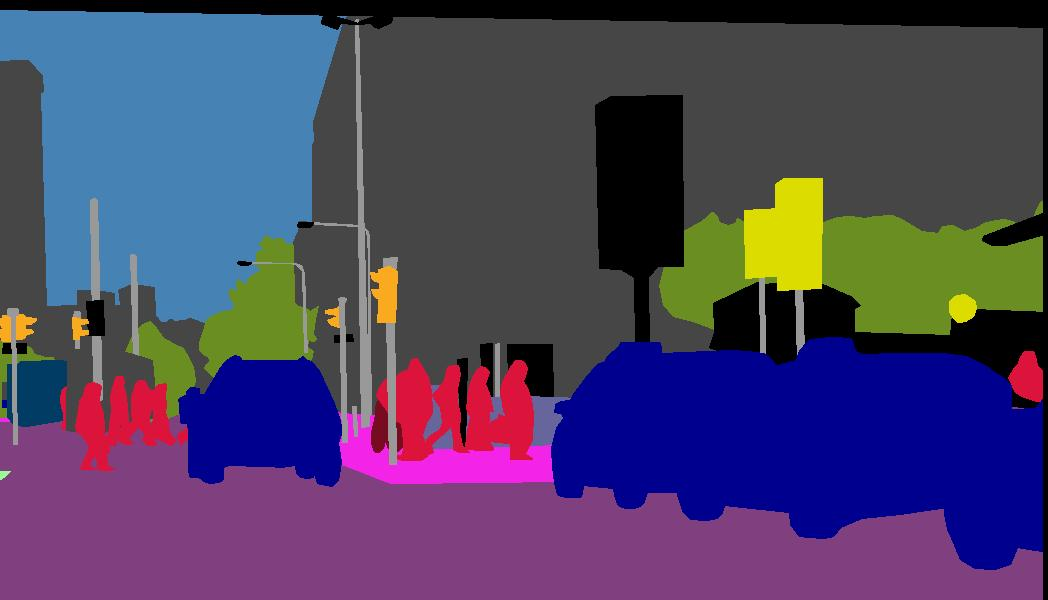
\includegraphics[width=0.3\textwidth]{fig/semantic_seg.jpg}
    }
    \subfloat[实例分割图]
    {
        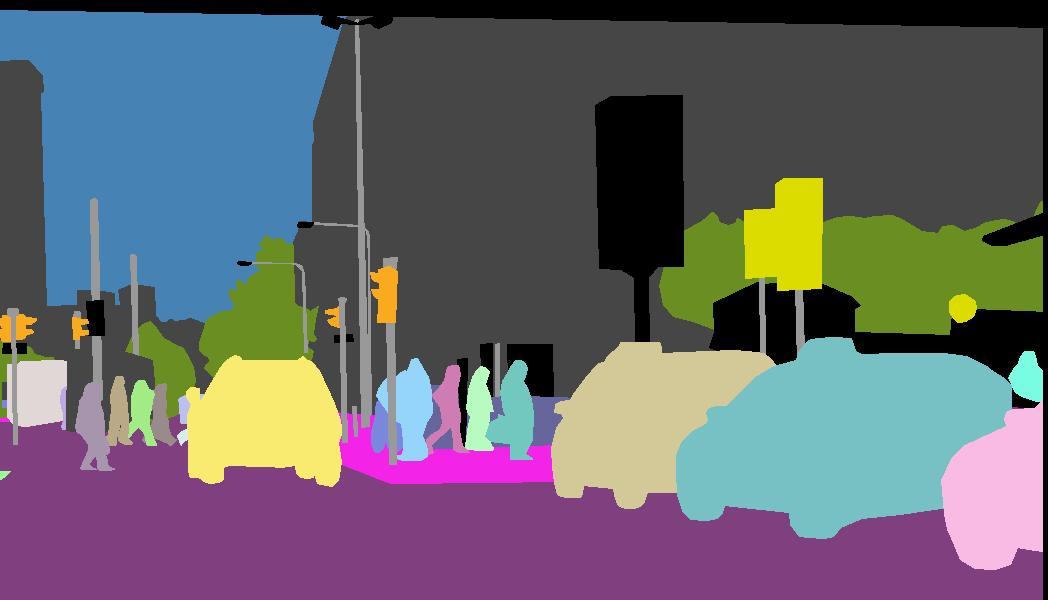
\includegraphics[width=0.3\textwidth]{fig/instance_seg.jpg}
    }
    \caption{语义分割与实例分割对比示意图\cite{kirillov2019}}
    \label{fig:seg}
\end{figure}

\subsubsection{医学图像特点}

% 考虑是否引用第一章某处内容
医学图像作为临床诊断与治疗决策的重要依据,具备区别于自然图像的一系列独特特点:

\begin{enumerate}
    \item 多模态性: 
    多模态性是医学图像最本质的特征之一,不同成像技术基于各自的物理机制产生图像,导致图像在分辨率、对比度、噪声特性等方面具有显著差异。例如,CT图像通过X射线衰减反映组织的密度信息,表现为良好的骨骼成像与高密度区域识别能力;MRI通过核磁共振原理获取图像,具有出色的软组织对比度,常用于脑部、脊髓及肿瘤成像。
    
    \item 高噪声和低对比度:
    相较于多数自然图像的高清晰度和高对比度,高噪声与低对比度问题在医学图像中普遍存在。受限于成像设备、器官运动等因素,医学图像常伴有伪影与模糊,如MRI中常见的运动伪影与磁敏感伪影、CT中的金属伪影。低对比度则体现在图像的病灶区域与周围正常组织在灰度分布上高度重叠,如肝脏与肿瘤组织;也常出现多个器官重叠或粘连的情况,如腹部CT图像中的脾脏与左肾的接触区域、脑白质与灰质区域。
    
    \item 解剖结构的拓扑复杂:
    自然图像的物体通常具有清晰空间分层(如“前景-背景”),而在医学图像中器官和组织常呈现多层嵌套(如肠管缠绕、血管穿透脏器)和动态形变(如呼吸导致的肺位移)。同时,自然物体的形状相对稳定,而人体解剖结构会因为个体差异、病理状态产生巨大形态变异,例如前列腺癌患者的腺体体积可膨胀至正常值的3倍。
    
    \item 数据获取和标注困难:
    医学图像的数据获取和标注远高于自然图像。成像成本高、病人隐私问题、罕见病例少等等因素导致医学图像的数据量通常只有数百数千张,甚至更少。同时高质量的可用于图像分割的医学图像需要具有多年经验的临床专家进行逐像素级精细勾画,且不同医生间的标注标准与经验存在差异,导致“标注者间差异”现象普遍存在。

\end{enumerate}

% 附图:自然图像+高噪声医学图像+复杂拓扑结构医学图像

上诉特点使得医学图像相较于自然图像有更高的复杂性,对其的自动分割任务不仅要求模型具备强大的特征表达与结构建模能力,还需应对多种极具挑战性的实际问题。

\subsubsection{医学图像语义分割挑战}

在数据具有多模态性和获取标注困难的情况下,跨模态泛化能力成为了衡量模型在医学图像语义分割性能的关键评估指标,一个鲁棒的能够适用于医学图像语义分割任务的模型应当能够在这种模态一致性不足和低数据量的情况下维持良好稳定的性能。而低对比度和解剖结构复杂的特点,对模型提出了更强的捕捉高分辨率细节并维持边缘清晰度的能力要求,许多早期病灶(如肺部结节、肝癌早期病变)和器官(如视网膜微血管)在图像中的所占面积比例极小,容易在下采样的过程中被忽略和抹除,模型需要能够在这种情况下对小目标进行精细分割。

除了受医学图像固有的复杂性影响,高实时性也是医学图像语义分割模型应当具备的能力,同时也是决定模型能否落地应用的重要门槛。在术中导航、放疗定位、超声实时识别等高时效性场景中,模型不仅要保证分割准确,还需在极短时间内完成推理,这同时也对模型的计算复杂度与硬件适配能力提出了极高的要求。

综上,面向于医学图像的语义分割算法和模型不仅有高分割精度和跨模态泛化的能力要求,还需要面对高实时性等的性能挑战。这种挑战也促使了大量的研究者进入医学图像语义分割领域进行探索,提出了诸多有效的分割算法和创新的网络结构与优化策略,这些工作将在下文中进行全面的介绍。

\subsection{传统分割方法概述}

% 结合医学图像中的应用阐述适用性和局限性,同时:删减内容!删减内容!

在相当长的一段时间内,或基于边界或基于区域的传统分割技术作为医学图像分析的基础,提供了一系列复杂性和适用性有所不同的方法。基于区域的分割方法依赖图像的空间特征,例如灰度和纹理,基于边界的分割方法则主要使用梯度信息来确定目标的边界。尽管阈值分割等传统方法在很多场景中有效\cite{xu2024},但其在跨模态、跨患者等任务中存在很大的局限性(详见第一章1.1节)。

传统分割方法现在来看已经“过时”,但作为深度学习方法兴起前的技术基础,其局限性为引入深度学习提供了动机。因此,本节将聚焦技术原理与医学应用适配性的角度,对阈值分割、边缘检测和聚类分割这三种最具代表性且广泛应用的传统分割方法进行概述总结。

\subsubsection{阈值分割}

阈值分割是图像分割中最基础、最广泛使用的技术之一,其核心思想是通过设定一个或多个灰度阈值,将图像像素进行二分类(如前景和背景):

\begin{equation}
B(x, y)=\left\{\begin{array}{ll}1, & \text { if } I(x, y) \geq T \\ 0, & \text { if } I(x, y)<T\end{array}\right.
\end{equation}

其中,$I(x, y)$表示图像在坐标$(x, y)$处的像素值,$B(x, y)$表示二值图像在坐标$(x, y)$处的像素值,$T$则是阈值。在图像处理中,阈值分割方法又可以细分为两大类:全局阈值法和局部阈值法。

全局阈值法假设整幅图像的背景与前景有明显的灰度差异,因此通过应用一个统一的阈值$T$来对图像进行分割。比较著名的全局阈值算法包括:Otsu法、迭代法和最小误差法。Otsu法通过最大化类间差异选取最优阈值;迭代法则初始估计一个阈值,然后迭代更新前景和背景的平均灰度值来计算新阈值直至收敛;最小误差法在基于图像前景和背景的像素灰度值呈正态分布的假设前提下,通过计算各分割区域的概率密度函数得到总分类误差并使误差最小化确定阈值。

相对于全局阈值法,局部阈值法假设图像具有不均匀的光照,因此针对每个像素的局部领域单独计算阈值$T$。较为常见的局部阈值算法包括:Niblack算法和Sauvola。Niblack通过计算每个像素上特定窗口内像素值的局部平均值和标准偏差,并利用平均值评估局部亮度、标准偏差衡量对比度和纹理来动态设定阈值:$ T=\mu+k \sigma $。Sauvola则在Niblack的基础上进行改进,将标准偏差的动态范围R引入阈值计算:$ T=\mu\left[1+k\left(\frac{\sigma}{R}-1\right)\right] $,从而更好地处理变化的背景和光照条件。

% 为这一段找一篇参考文献
凭借其计算简单、易于实现等优点,阈值法在灰度分布清晰、对比度明显的医学场景中广泛应用,如X射线骨骼分割、肺部CT气腔提取等初步分割任务。但是由于依赖图像整体灰度分布,在面对光照不均、伪影干扰、组织边界模糊以及病灶与背景对比度微弱等复杂医学图像时,阈值法往往出现误分割、边界锯齿或目标遗漏等问题。此外,阈值法也难以处理多目标或多组织分割任务,需要手动调节多个阈值,增加了流程复杂度。

\subsubsection{边缘检测}

% 记得插入参考文献

边缘是指两个均匀区域之间的边界,表现为图像中像素强度的局部突变,而边缘检测的核心就在于识别定位图像中像素强度突变的位置。

图像边缘具有两个基本特性:方向与幅值。沿着边缘方向,像素值的变化往往较为平缓;而在垂直于边缘方向,像素值的变化则较为剧烈。基于这一特性,通过应用一阶和二阶微分算子与图像像素值矩阵进行卷积运算,精确计算各像素点的梯度变化或曲率,从而实现提取边缘特性。

常见的一阶微分算子包括Roberts交叉算子、Prewitt算子、Sobel算子以及Canny边缘检测器。Prewitt算子与Sobel算子均采用像素邻域差分法进行边缘检测。其中,Prewitt算子对边缘方向具有更高的敏感性,而Sobel算子则通过改进的噪声抑制能力获得更优性能,但代价是可能导致边缘轻微模糊。Canny算子作为多阶段边缘检测算法的典型代表,以高精度著称,不仅能有效抑制噪声干扰,还可实现边缘的准确定位,但其计算复杂度显著高于其他算子。

二阶微分算子如Laplacian算子和LoG算子同样被广泛采用。基于二阶导数的Laplacian算子对图像细节具有突出增强作用。尽管该算子易受噪声影响,但在细微特征增强方面表现卓越。LoG算子通过高斯平滑预处理与Laplacian算子的协同作用,有效降低了噪声干扰,特别适用于噪声敏感环境下需要精确定位边缘的应用场景。

% 插入参考文献
如表~\ref{tab:edge_detectors}所示,传统边缘检测算子因其算法特性各异而展现出不同优缺点,因此也具有不同的应用价值和局限性,适用于不同的应用场景。Roberts算子凭借其计算效率高的优势,适用于病理切片等显微图像的快速分析,但对噪声敏感的特性使其在CT/MRI等模态中易产生伪边缘。Prewitt算子和Sobel算子因其通过加权增强边缘方向性,故适用于如X光胸片肋骨等轮廓清晰的图像分割,但难以处理边界模糊的情况;Canny算子则因其具备噪声抑制、边缘连接性强等特性,能精确定位MRI脑肿瘤边界,却存在参数调优复杂、计算耗时等问题。Laplacian算子对微小钙化点检测敏感,却完全无法抵抗超声斑点噪声的干扰。LoG算子虽能实现多模态边缘增强,但其高昂的计算成本限制了临床应用。

\renewcommand{\tabularxcolumn}[1]{m{#1}}
\newcolumntype{C}{>{\centering\arraybackslash}X}
\begin{table}[!htbp]
\centering
\caption{不同边缘检测算子的优缺点比较}
\label{tab:edge_detectors}
\begin{tabularx}{\textwidth}{@{}C C C@{}}
\toprule
\textbf{算子} & \textbf{优点} & \textbf{缺点} \\
\midrule
Roberts & 计算简单 & 对噪声敏感,边缘定位不准 \\
\addlinespace
Prewitt & 对边缘方向敏感 & 对噪声敏感,边缘较模糊 \\
\addlinespace
Sobel & 抑制噪声 & 边缘易过平滑\\
\addlinespace
Canny & 边缘检测精度高,抗噪性强 & 计算复杂,依赖参数调优\\
\addlinespace
Laplacian & 能定位边缘中心 & 抗噪性极差,无方向信息 \\
\addlinespace
LoG算子 & 抗噪性强且边缘定位准 & 计算量大,可能丢失细边缘 \\
\bottomrule
\end{tabularx}
\end{table}

\subsubsection{聚类分割}

聚类分割通过将相似特征的像素归类至同一簇实现图像分割,其核心在于定义合理的相似性度量。根据聚类策略的不同,主要分为层次聚类与划分式聚类两类。

在层次聚类方法中,簇的生成通常通过一种迭代式的模式划分过程实现,该过程可以采用自顶向下或自底向上的策略,通过构建树状图生成每个簇仅包含单一数据实体的层级簇结构来完成聚类任务。尽管层次聚类方法具有良好的可解释性与层级结构建模能力,但在医学图像语义分割场景下存在若干显著缺陷:

\begin{enumerate}
    \item 贪心策略限制:样本一旦归类无法修正,噪声或离群点易导致错误累积。
    \item 计算复杂度高:时间复杂度达$O(n^3)$,难以处理大规模医学数据(如全脑MRI体素)。
    \item 预设参数敏感:需人工设定簇数或终止条件,难以自适应复杂解剖结构(如肿瘤浸润区域)。
\end{enumerate}

划分式聚类方法(如k-means算法、模糊c均值算法)则通过优化目标函数,将数据样本划分为若干个彼此独立的簇,从而增强簇内样本间的相似性,并尽可能降低簇间差异,从而寻求最优的聚类配置。其主要优势在于其具备迭代优化能力,能有效适应数据结构的变化。但其局限性也同样突出:

\begin{enumerate}
    \item 初始条件敏感:随机初始簇中心可能导致结果不稳定。
    \item 形状假设偏差:默认球形簇分布,难以分割非凸结构(如树枝状血管网络)。
    \item 噪声干扰:离群点易扭曲簇中心(如超声图像中的斑点噪声)。
\end{enumerate}

\subsection{基于深度学习的语义分割技术}

深度学习作为机器学习与人工智能领域的重要研究方向,其核心在于通过深度神经网络模拟人脑学习机制,从海量数据(语音、文本、图像等)中以无监督方式自动提取特征表征。神经网络通过大量互连的神经元,从结构、实现机理和功能上模拟人脑神经网络,每个神经元可视为基础信息处理单元,通过层级化连接形成完整的网络架构\cite{qiu2020nndl}。该架构的出现使得端到端图像处理成为可能,当网络隐层扩展至多层结构时即形成深度学习范式。在计算机视觉领域,深度学习已成功应用于数据降维、手写体识别、模式识别等方向,尤其在图像识别、图像修复、图像分割、目标追踪及场景解析等任务中展现出卓越性能。

\subsubsection{卷积神经网络}

% 章节脉络:
% 介绍卷积神经网络 -> 介绍FCN模型 -> FCN的成功和局限
% 1.介绍卷积神经网络:历史及基本介绍 -> 技术细节 -> CNN如何正式引入图像分割领域
% 2.介绍FCN模型: 模型架构 -> 如何完成语义分割
% 3.成功和局限: 成功在哪 -> 局限在哪

% 1.1
卷积神经网络是深度学习与图像处理技术相结合的经典网络结构,作为深度学习技术领域最具代表性的神经网络之一,在图像分析与处理领域取得了诸多突破性进展。例如,在学术界广泛使用的标准图像标注集ImageNet上,基于卷积神经网络的特征提取与分类、模式识别等研究成果颇为丰硕。

受生物学上Hubel等人\cite{hubel1962}提出的感受野的概念启发,1980年Fukushima\cite{fukushima1980}提出了神经认知机,被视为卷积神经网络的首次实现网络。与全连接层前馈网络不同的是,卷积神经网络通过交叉堆叠卷积层、池化层和全连接层形成前馈神经网络。大量的卷积层和池化层使得网络可以共享前层网络不同位置的特征映射权重,并利用空间相对关系来大大减少网络的参数量,这与大脑视觉神经元只能对视网膜上某一特定区域的光刺激产生反应的机制类似。同时,结构特性带来的一定程度上的平移、缩放和旋转不变性,使得卷积神经网络在图像和视频分析任务上具有远超其他神经网络模型的准确率。

% 1.2
图~\ref{fig:cnn}展示了一般卷积网络的整体结构,其中包含若干个卷积核和非线性激活函数的卷积层是卷积神经网络的核心组成部分。所有卷积核对输入数据进行并行卷积运算得到卷积线性输出,之后再经过激活函数就得到了卷积层的输出\cite{Goodfellow-et-al-2016}。

\begin{figure}[htbp]
    \centering
    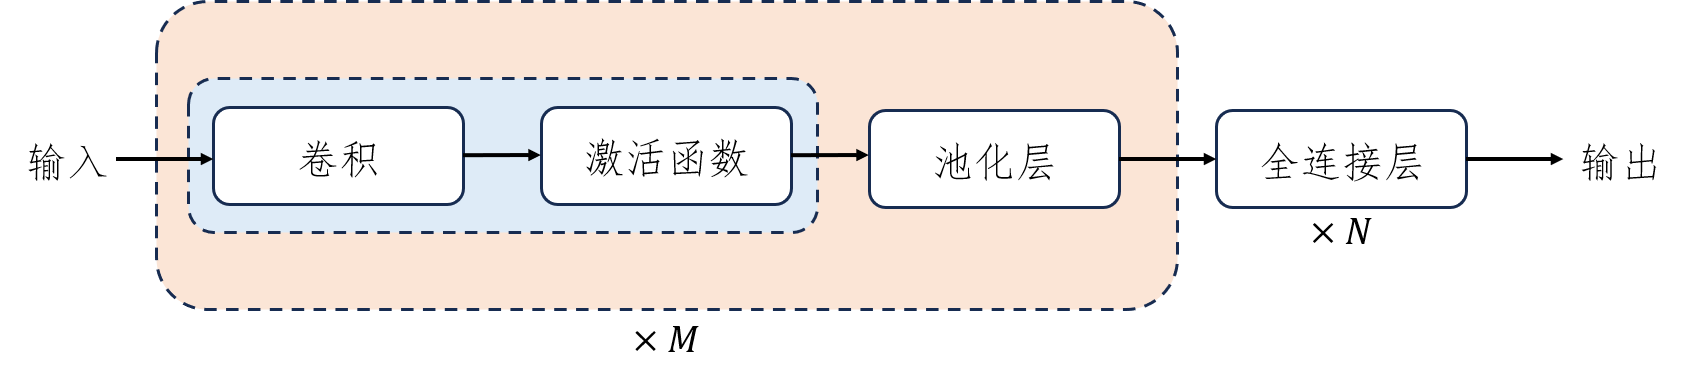
\includegraphics[width=\textwidth]{fig/cnn_frame.png}
    \caption{卷积网络的整体结构}
    \label{fig:cnn}
\end{figure}

在图像处理中最常见的卷积运算是二维卷积运算,即输入数据是二维张量:

\begin{equation}
    O(i, j)=(I * K)(i, j)=\sum_{m} \sum_{n} I(m, n) K(i-m, j-n)
\end{equation}

其中$*$表示二维卷积运算,图~\ref{fig:2dcnn}展示了其计算过程。$I$和$K$都是二维张量,$ K \in \mathbb{R}$表示可学习的二维卷积核权重向量,$I \in \mathbb{R}$表示输入的二维图像数据,$(x, y)$代表像素点坐标,$(m, n)$代表输入图像的尺寸。

\begin{figure}[htbp]
    \centering
    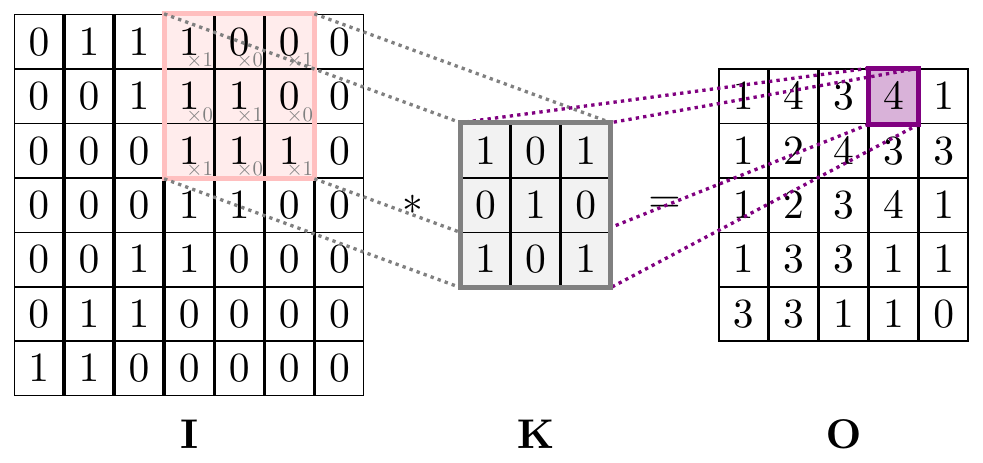
\includegraphics[width=0.7\textwidth]{fig/2dcnn-1.png}
    \caption{二维卷积运算}
    \label{fig:2dcnn}
\end{figure}

% 2.1
在全卷积网络(Fully Convolution Network, FCN)出现之前,诸如GoogLeNet、ResNet等采用卷积神经网络构建的模型主要应用于图像分类和识别,在图像语义分割领域缺乏有针对性的、表现优异的卷积神经网络模型,而FCN是首个开创性将卷积神经网络引入图像语义分割领域的网络模型\cite{shelhamer2016}。

如图~\ref{fig:fcn_frame}所示,作为后续诸多分割模型模型的基础架构,FCN借鉴了VGG网络的层次化设计,可以支持任意尺寸的输入图像,采用逐像素交叉熵损失进行反向传播,整个网络端到端训练输出与输入同尺寸的逐像素类别图。

\begin{figure}[htbp]
    \centering
    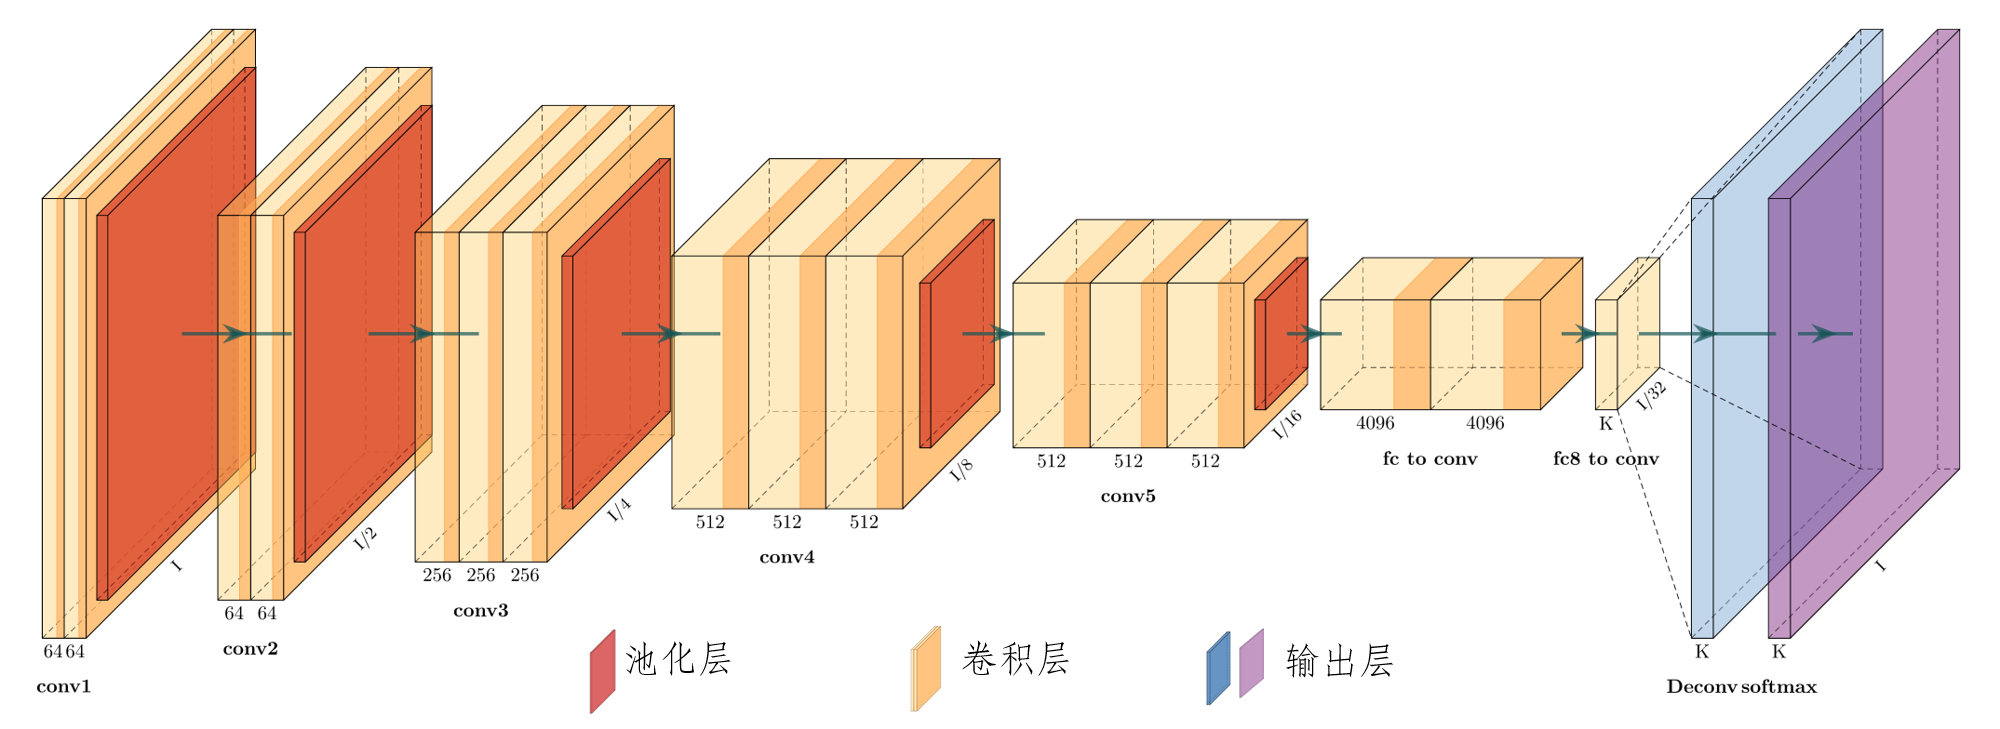
\includegraphics[width=\textwidth]{fig/fcn_frame.png}
    \caption{全卷积网络模型架构}
    \label{fig:fcn_frame}
\end{figure}

% 2.2
与传统分割模型和卷积神经网络通过若干个全连接层得到一个全局类别标签不同的是,FCN中的全连接层被全部替换为了卷积层,输入图像首先经过卷积层提取特征和上下文信息;之后经过反卷积层逐步从低分率特征图恢复到原分辨率图像。其中,卷积层、反卷积层也称为编码器、解码器,这样的网络结构也称为编码器-解码器结构。

% 3.1 + 3.2
FCN模型是语义分割领域的里程碑并开启了“全卷积”时代,后续的SegNet、Deeplab和U-Net等模型皆在此框架上演进。全卷积的架构不仅解决了全连接层会破坏空间信息导致模型整体性能下降的问题,还打破了输入尺寸的限制,使大面积图像一次向前即可完成推理。然而,如图~\ref{fig:fcn_pre}所示,由于过深的卷积下采样,这使得FCN网络的分割结果存在边界粗糙、细节丢失等问题,虽然Long等人尝试通过跳跃连接的方式,将卷积层下采样的结果与上采样的结果进行特征融合以缓解问题,但对于医学图像语义分割这种图像包含小器官小目标且高精度分割要求的任务,FCN网络的分割结果还远远无法满足要求。

\begin{figure}[htbp]
    \centering
    \subfloat[原图]
    {
        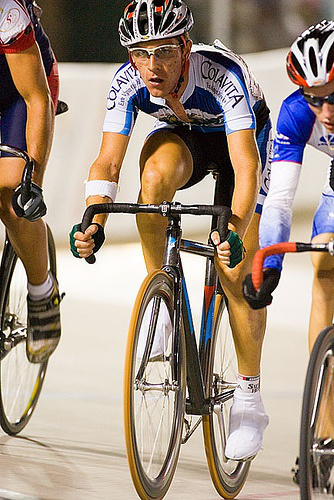
\includegraphics[width=0.25\textwidth]{fig/img4.png}
    }
    \subfloat[原图分割图]
    {
        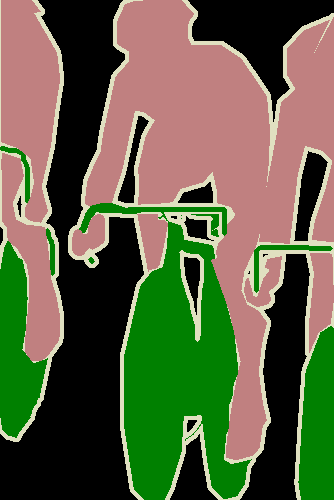
\includegraphics[width=0.25\textwidth]{fig/gt4.png}
    }
    \subfloat[FCN预测分割图]
    {
        
\includegraphics[width=0.25\textwidth]{fig/predsf4.png}
    }
    \caption{原图分割图与FCN预测分割图的差别\cite{shelhamer2016}}
    \label{fig:fcn_pre}
\end{figure}

\subsubsection{U-Net网络}
% 章节脉络:模型架构 -> 模型医学图像优势 -> 模型存在的局限性
% 模型架构:整体架构 -> 各部分架构及其左右
% 模型优势:为什么如此有效 -> 在医学图像语义分割领域取得的具体成果
% 局限性: 模型局限 -> 实践局限

% 1.1
受FCN网络的启发,Ronneberger等人在其全卷积架构和解码器-编码器网络结构设计的基础上提出了U-Net网络,这个专门解决为医学图像语义分割任务而出现的模型在出现后广泛被应用于医学图像语义分割,也成为了后续在此基础上进行改进的U-Net变体模型的基线模型。

\begin{figure}[htbp]
    \centering
    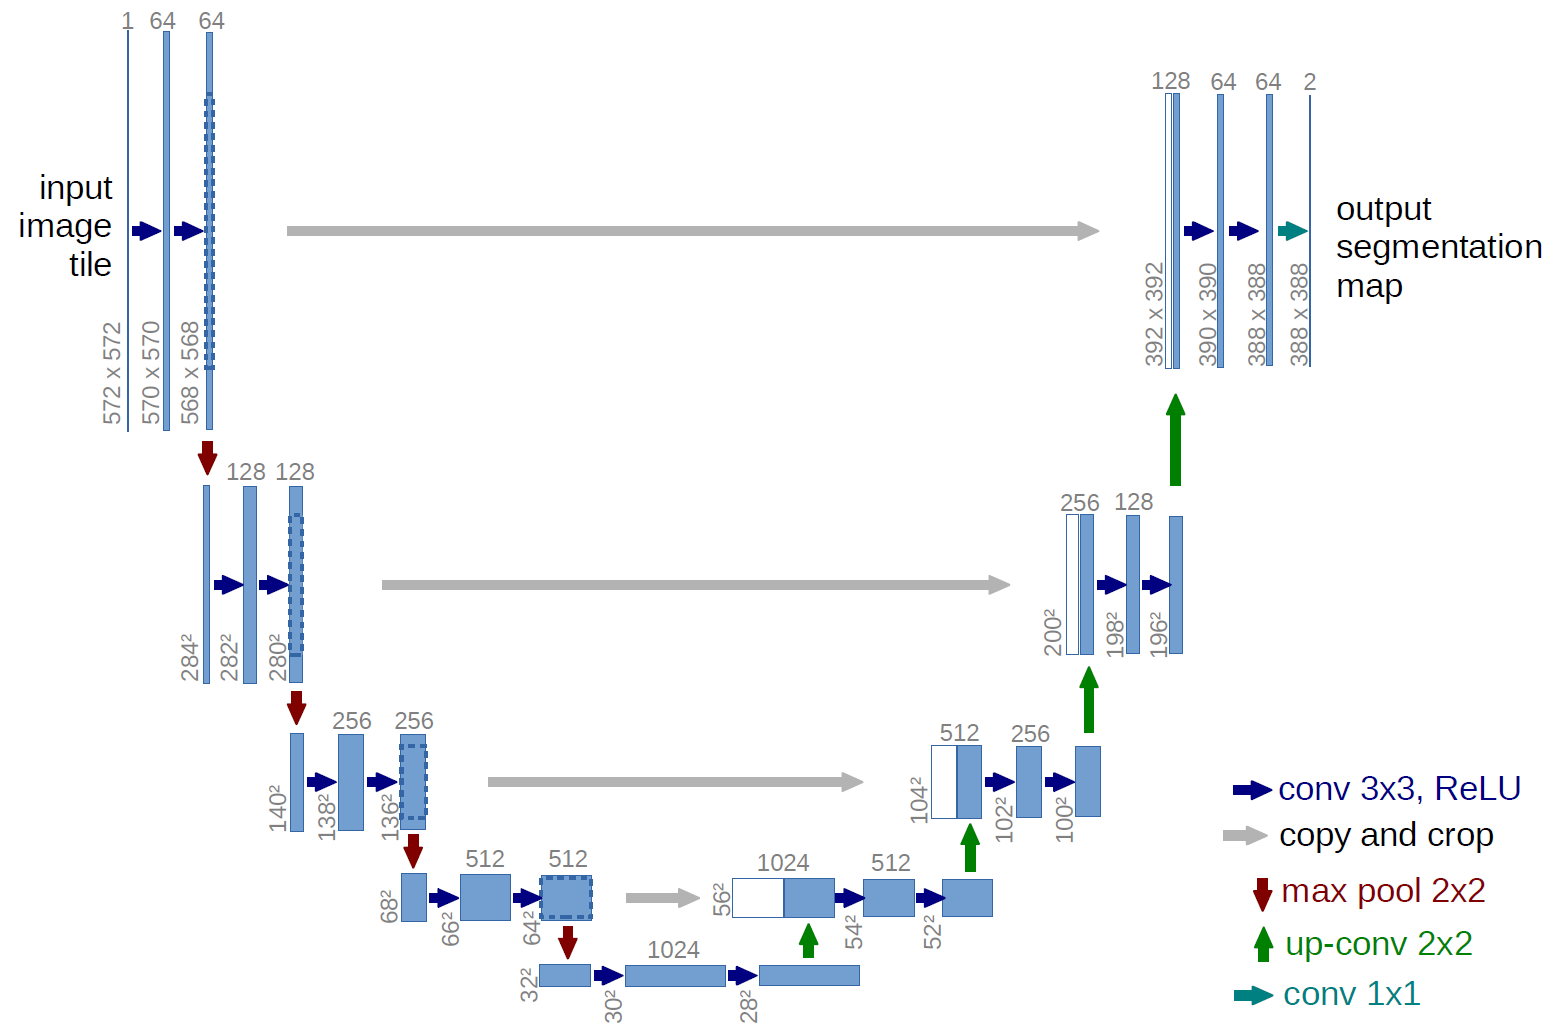
\includegraphics[width=0.8\textwidth]{fig/u-net-architecture.png}
    \caption{U-Net网络架构\cite{ronneberger2015}}
    \label{fig:unet_frame}
\end{figure}

图~\ref{fig:unet_frame}展示了U-Net网络的网络架构,由两部分构成:

\begin{enumerate}
    \item 收缩路径:也称下采样路径。由多个卷积层和池化层组成一个下采样模块,用于提取语义与上下文特征。
    \item 扩张路径:也称上采样路径。由转置卷积层和多个卷积层组成一个上采样模块,用于逐步恢复特征图的空间分辨率。
\end{enumerate}

% 1.2
可以看出,U-Net网络结构与FCN相似,均采用了编码器和编码器以及跳跃连接的拓扑结构。有所区别的是,FCN缺少严格配对的收缩路径和扩张路径,仅在三个尺度上将早期特征“逐像素相加。U-Net在这个基础上构建了与收缩路径一一对应的扩张路径,形成了经典的对称“U”字结构。每个编码器和解码器相对应的层都进行输出拼接,再经过两个卷积层卷积对拼接特征图进行特征融合。

这种创新式的跳跃连接方式,将收缩路径上高分辨率的上下文信息传递到深层网络,使得模型能够复用低层细节特征和高层语义信息,从而实现对目标的精准定位。同时,每次上采样后都采用3×3卷积连续细化的方式,使得像素级定位更加准确,特别适合需要像素分割精度的医学图像语义分割任务。凭借着U-Net模型,Ronneberger等人在ISBI细胞跟踪竞赛中以远超其他模型的性能表现大获成功\cite{ronneberger2015}。
\section{基准U-Net模型设计与实现}

\subsection{数据集准备与预处理}

\subsubsection{ISBI皮肤镜影像数据集}

ISBI皮肤镜影像数据集(2018年)由国际皮肤影像协作组织(International Skin Imaging Collaboration, ISIC)联合Memorial Sloan Kettering Cancer Center、University of Queensland等多家机构共同构建,并作为ISIC 2018皮肤病变识别挑战赛(ISIC Challenge 2018)的官方数据资源\cite{codella2019skinlesionanalysismelanoma}。该挑战共设立了三项任务:皮肤病变分类、像素级病变区域分割以及病变属性预测,数据集也据此提供了相应的图像与标注文件。

ISIC 2018数据集作为目前最具影响力的皮肤镜数据集之一,广泛用于皮肤病变分割与分类模型的基准测试。数据集总共包含2594张RGB三通道皮肤镜图像,图像格式为JPEG或PNG,分辨率在600×450至6748×4499像素之间,保留了丰富的病变细节特征(如色素网、结构不规则性、色斑边缘模糊等),图像采集过程遵循标准化的成像协议(如偏振光皮肤镜)。除图像本体外,每张图像还附带包括患者年龄、性别、病变解剖部位等在内的临床元数据,具备一定的多模态分析潜力。

在标注方面,数据集提供由皮肤科专家精确勾画的像素级病变掩膜用于病变区域分割任务训练,掩膜的标注一致性通过交叉验证确认(Kappa 系数大于 0.82)。同时,整个数据集按照任务需求被官方划分为训练集(2,000 张,含掩膜和标签)、验证集(300 张,仅标签)与测试集(294 张,无公开标注,仅用于模型评估)。

为确保输入数据的一致性与模型训练的稳定性,本研究对ISIC 2018皮肤镜影像数据集中的图像及其对应的掩膜进行了标准化预处理。所有RGB皮肤镜图像统一归一化至$(0,1)$范围,掩膜转换为双通道概率标签(0-背景,1-病变),为后续使用基于概率分布的损失函数(如交叉熵损失、Dice损失)提供结构支持。

为确保训练过程的可控性与评估结果的可靠性,数据集严格遵循官方划分比例(训练集:验证集:测试集=70\%:15\%:15\%),通过随机分层抽样确保分布一致性,避免评估偏差。

\subsubsection{LiTS肝脏CT数据集}

LiTS(Liver Tumor Segmentation)数据集是由MICCAI 2017肝脏肿瘤分割挑战赛(Liver Tumor Segmentation Challenge 2017)发布的医学影像公开数据集,由来自全球多家权威医疗机构提供的腹部增强CT扫描组成,涵盖130例临床病例,包含多种肝脏病理状态,包括肝细胞癌、转移性肿瘤、胆管细胞癌等\cite{Bilic_2023}。所有图像数据均采用静脉期CT成像,层厚范围为1–5mm,横断面矩阵分辨率为512×512,体素间距在0.6–1.0 mm之间(存在一定程度的各向异性)。成像窗宽窗位统一设定为肝脏窗(窗宽150–200 HU,窗位约-50–50 HU),以增强肝实质与病灶之间的密度对比。

在标注方面,数据集中每一病例均由三位经验丰富的放射科专家进行独立标注,提供像素级肝脏与肿瘤分割掩膜。标注一致性通过Dice系数(平均大于0.92)和Hausdorff距离(平均小于5 mm)进行验证,部分病例还附带有病灶的病理学分型标签。

LiTS 2017数据集的挑战性体现在多方面:其一,肝脏轮廓复杂、变异性大,且边界常与胃肠道等邻近脏器重叠,导致区域判别困难;其二,肿瘤病灶形态异质性强(如结节型、融合型、浸润型),并存在大小悬殊、边界模糊、低密度病灶等不利因素;此外,呼吸运动伪影与层间不连续性也显著增加了分割任务的难度。

在模型训练前,本研究对LITS 2017肝脏CT数据集进行了系统性预处理,以确保数据一致性与模型输入的可靠性。所有CT图像以伪彩色映射形式统一读取为RGB三通道格式,并转换为浮点张量,数值范围归一化至$(0,1)$;对应的单通道掩膜(0表示背景,1表示肝脏及肿瘤区域)同步转换为张量格式,针对二分类任务需求,掩膜进一步编码为双通道概率标签(通道0为背景概率,通道1为前景概率),以适配基于概率分布的损失函数。数据集严格遵循预定义划分策略,通过固定随机种子生成可复现的训练集、验证集与测试集分配方案。此外,文件名经匿名化处理,患者隐私信息完全脱敏,符合医学伦理规范。整体流程通过标准化映射、严格划分与一致性校验,为肝脏肿瘤分割任务构建了高鲁棒性的数据基础。

\subsubsection{BraTS脑肿瘤MRI数据集}

BraTS(Brain Tumor Segmentation)2020 数据集由 MICCAI 组织联合宾夕法尼亚大学、慕尼黑工业大学等多家国际顶尖医学与工程研究机构共同构建,作为年度脑肿瘤分割挑战赛的重要基准数据资源\cite{menze2015}。该数据集专注于胶质瘤(包括高级别胶质瘤HGG与低级别胶质瘤LGG)MRI图像的分割任务,广泛用于评估多模态影像分割算法的性能与鲁棒性。

数据集中共包含 369例患者的多模态MRI扫描数据,每例数据均包含四种标准MRI模态:T1加权(T1)、T1对比增强(T1ce)、T2加权(T2)以及液体衰减反转恢复序列(FLAIR)。所有图像均经过统一预处理流程,包括:

\begin{enumerate}
    \item 各向同性重采样至1.0×1.0×1.0 mm³体素分辨率
    \item N4偏场校正以消除非均匀磁场引起的信号漂移
    \item 跨模态配准,确保不同模态间空间对齐一致。
\end{enumerate}

在数据标注方面,每例数据均提供由神经放射学专家联合标注的像素级三维分割掩膜,标注内容涵盖:

\begin{enumerate}
    \item 增强肿瘤区域(Enhancing Tumor,ET):表现为对比增强T1序列中具有强化表现的病灶区域;
    \item 肿瘤核心(Tumor Core,TC):包括坏死区域、实性肿瘤与增强部分;
    \item 肿瘤整体(Whole Tumor,WT):包括肿瘤核心与周围水肿区域。
\end{enumerate}

BraTS 2020数据集的主要挑战包括:(1)肿瘤组织的高度异质性,如增强区与坏死区边界模糊;(2)小体积或卫星灶的检测难度高,极易被误判或遗漏;(3)多模态之间的病灶表征差异显著,对模型特征融合能力提出更高要求。

为构建高效且可复现的脑肿瘤分割数据管线,本研究基于BraTS 2020数据集设计了系统化预处理流程。首先,所有病例按目录名排序并剔除损坏样本,采用两级随机划分策略:10\%病例作为独立测试集,剩余病例在固定随机种子控制下进一步分为训练集(70\%)与验证集(20\%),病例ID分配方案持久化为JSON文件以确保实验可复现性并避免数据泄漏。

不同于ISBI 2018和LiTS 2017数据集,针对BraTS数据集是多模态数据的情况,仅采用FLAIR和T1对比增强两种模态组合作为输入序列,有研究表明对于脑肿瘤语义分割任务,这种序列组合是最佳的组合选择\cite{buchner2023}。此外,所有输入数据逐例归一化至$(0,1)$范围以消除扫描设备差异,并遍历三维体积数据的轴向切片,剔除无标注信息的空白切片(分割掩膜全零),缓解类别极端不平衡问题;对原始标签(增强肿瘤、肿瘤核心、坏死区)按临床需求重映射为统一类别体系,并转换为多通道one-hot编码,适配交叉熵损失与Dice损失的监督需求。

总结来说,每张切片被组织为2-通道输入(FLAIR + T1ce)和4通道one-hot标签,按批次送入数据流水线。管线支持随机打乱、动态批量组装、并行预取和可选重复迭代,从而在保证 I/O 吞吐的同时充分混洗样本。

\subsection{基准U-Net模型构建}
%详细描述U - Net模型的构建过程,包括网络层的搭建、损失函数的选择(如Dice损失函数)等。
%训练过程中的参数设置,如学习率、批量大小、训练轮数等。
本研究在经典U-Net框架的基础上实现了基准U-Net模型的构建,用以评估后续改进策略的真实收益。模型构建包括网络层的搭建、损失函数的涉及和优化器的选择。

\subsubsection{网络层}

图~\ref{fig:unet_ushape}展示了本研究搭建的基准U-Net模型的模型架构,网络采用对称的编码器—解码器结构:

编码端连续堆叠四级特征抽取单元,每一级由两层3×3有填充卷积与ReLU激活组成;特征通道数以32为起始,在每次下采样后按1∶2的比例递增(即32→64→128→256)。空间下采样通过2×2最大池化实现,使特征图尺寸依次减半,从而在更大的感受野上编码语义信息。

解码端采用与编码端对称的结构,对最深层特征进行转置卷积上采样,并与对应级别的编码器输出进行特征级串接后,执行两层卷积+激活以还原局部细节。此跳跃连接在保持全局上下文同时弥补高分辨率细节缺失,是U-Net能够兼顾定位精度与类别判别力的关键机制。最终输出层采用1×1卷积,将通道数映射为$C$($C$为分割图的像素类别数),输出未经激活直接送入损失函数计算,以便在训练阶段灵活选择Sigmoid或Softmax型损失。

\begin{figure}(htbp)
    \centering
    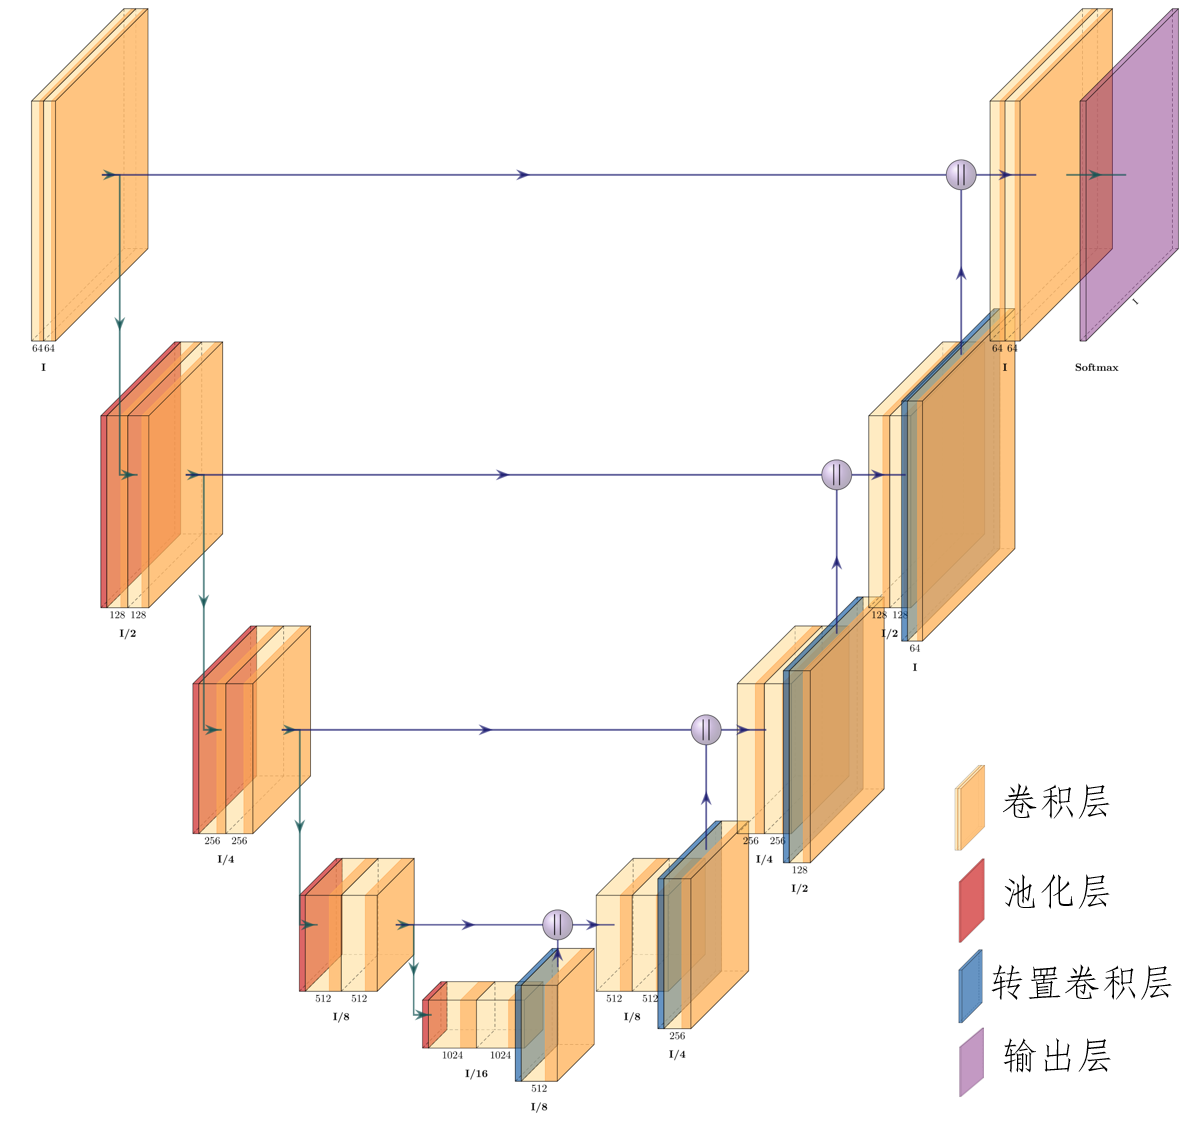
\includegraphics[width=0.6\textwidth]{fig/Unet_ushape.png}
    \caption{fig:unet_ushape}
    \label{基准U-Net模型的模型架构}
\end{figure}

上述网络拓扑及通道配置均采用Pytorch框架实现,对应的实现要点可在附录A中进一步查证。

\subsubsection{损失函数的设计}

在损失函数的设计上,本文采用Dice – Cross-Entropy混合损失(以下简称混合损失),即以相等权重线性叠加Dice损失与像素级交叉熵(CE)损失,以充分兼顾类别不平衡下的区域重叠度优化与梯度稳定性。设网络输出的类别概率图(像素总数为$N$)为:$ P=\left\{p_{i}\right\}_{i=1}^{N} $,真实分割掩膜为$ G=\left\{g_{i}\right\}_{i=1}^{N} $,其中$ p_{i} \in[0,1], g_{i} \in\{0,1\}$分别是像素$i$的前景概率和真实标签。则:

\begin{equation}
    \mathcal{L}_{\text {Dice }}=1-\frac{2 \sum_{i=1}^{N} p_{i} g_{i}}{\sum_{i=1}^{N} p_{i}+\sum_{i=1}^{N} g_{i}+\varepsilon}
\end{equation}

\begin{equation}
    \mathcal{L}_{\mathrm{CE}}=-\frac{1}{N} \sum_{i=1}^{N}\left[g_{i} \ln \left(p_{i}\right)+\left(1-g_{i}\right) \ln \left(1-p_{i}\right)\right]
\end{equation}

\begin{equation}
    \mathcal{L}_{\text {mix }}=0.5 \mathcal{L}_{\text {Dice }}+0.5 \mathcal{L}_{\mathrm{CE}}
\end{equation}

其中$ \varepsilon=10^{-6} $用于数值平滑以防零分母。Dice项直接对预测与标注的重叠区域进行归一化度量,能在小体积病灶场景下显著提升召回;交叉熵项则提供像素级对数似然的密集监督,改善早期训练阶段梯度稀疏、收敛震荡等问题。

\subsubsection{优化器的选择}

优化器采用Adam随机梯度下降算法,其一阶自适应动量可在早期快速探索有效学习率区间,同时在震荡平衡阶段保持较小更新幅度。初始学习率设定为$ 1.0 \times 10^{-4} $,一阶、二阶动量系数沿用默认值$ \beta_{1}=0.9, \beta_{2}=0.999 $。

\subsection{训练策略与评估指标}

\subsubsection{训练策略}

模型的训练均在Kaggle平台进行,采用Kaggle平台提供的NVIDIA P100 (16 GB) 单卡进行模型加速训练。

为了避免训练后期进入平台期,附加 Reduce-on-Plateau 学习率调度策略:当验证集指标在 10 个 epoch 内无显著提升时,将学习率衰减为原值的 0.5;最低学习率限定在$ 1.0 \times 10^{-6} $,防止数值下溢而不再更新参数。当学习率因多次衰减而触碰下限时,若模型仍无改善,则提前终止训练以节省算力。

训练超参数经预实验网格搜索确定:批量大小根据数据集的规模和大小确定,完整训练周期设置为100epoch,保证验证过程与训练同步,本研究在每个 epoch 结束后立即于验证集评估 Dice 系数并记录最优权重;测试集仅使用单尺度推断,不采用多尺度或模型集成,确保基准模型公平、简洁、可复现。

\subsubsection{评估指标}

在医学图像分割研究中,模型输出通常为与输入图像同尺寸的二值概率图,衡量其与专家标注掩膜之间的相似程度是评价算法优劣的关键。单一指标无法满足同时反映检测率、误诊率和重叠精度的要求,多指标可立体呈现模型表现。因此,在本研究中,我们以混淆矩阵四要素(真阳性TP、真阴性TN、假阳性FP、假阴性FN)为基础,记录Accuracy、Precision、Recall、Specificity、F1-Score、Dice系数与Jaccard指数七项评估指标。下面逐一给出这些指标的定义、公式及其评价意义。

准确率Accuracy表示正确预测的样本占总样本的比例,是最直观的分类性能指标:

\begin{equation}
    \mathrm{Accuracy}=\frac{TP+TN}{TP+TN+FP+FN}
\end{equation}

Accuracy直观反映模型的综合判断能力,但在病灶面积远小于背景时,Accuracy易受TN主导,可能高估模型质量,因此仅作为参考基线。

特异性Specificity表示实际为负类的样本中被正确预测的比例,衡量模型识别阴性样本的能力:

\begin{equation}
    \mathrm{Specificity}=\frac{T N}{T N+F P}
\end{equation}

在医学任务中,高特异性可减少健康组织被误判为病变的风险(如避免正常脑组织被误分割为肿瘤),提升结果的可信度,与 Recall 形成互补。

Jaccard指数(IoU)计算预测与真实标签的交集与并集的比值,是分割任务的经典指标:

精确率Precision表示预测为正类的样本中实际为正类的比例,反映模型的预测可靠性:

\begin{equation}
    \mathrm{Precision}=\frac{T P}{T P+F P}
\end{equation}

Precision反映模型整体预测正确性,但在类别极度不平衡时(如背景像素占比90\%以上),可能高估性能(例如模型仅预测背景即可获得高准确率),需结合其他指标综合判断。

召回率Recall召回率表示实际为正类的样本中被正确预测的比例,反映模型对正类样本的覆盖能力:

\begin{equation}
    \mathrm{Recall}=\frac{T P}{T P+F N} 
\end{equation}

高召回率意味着模型能有效捕捉病变区域(减少漏检),在早期诊断(如癌症筛查)中至关重要,但需平衡精确率以避免过度预测。

F1-Score是Precision与Recall的调和平均数,综合衡量模型在正类样本上的分类能力,尤其适用于类别不平衡场景:

\begin{equation}
    \mathrm{F} 1=\frac{2 T P}{2 T P+F P+F N}=2 \cdot \frac{\text { Precision } \times \text { Recall }}{\text { Precision }+ \text { Recall }}
\end{equation}

F1分数可以避免仅关注单一指标(如高精确率但低召回率),在医学图像分割中(如肿瘤区域占比小),能更均衡评估模型对正类(病变区域)的捕捉能力与预测准确性。

Dice系数衡量预测结果与真实标签的重叠程度,是医学图像分割的核心评估指标:

\begin{equation}
    \mathrm{Dice}=\frac{2 T P}{2 T P+F P+F N}=\frac{2 \times|A \cap B|}{|A|+|B|}
\end{equation}

其中,A为预测区域,B为真实区域。Dice系数直接衡量空间重叠,对不平衡数据敏感度低,能有效评估模型对病灶轮廓的捕捉精度,尤其适用于小目标分割任务(如脑肿瘤核心)。

\begin{equation}
    \mathrm{Jaccard}=\frac{T P}{T P+F P+F N}=\frac{|A \cap B|}{|A \cup B|}
\end{equation}

其中,A为预测区域,B为真实区域。Jaccard指数严格量化重叠区域的比例,对分割边界的轻微偏移敏感,常用于评估模型在复杂解剖结构(如肿瘤浸润区域)中的细节保留能力,在多模型比较时可提供更保守的评估视角。
\section{改进的U-Net模型设计}

尽管U-Net网络的跳跃连接能够有效地结合浅层和深层特征,但在处理小目标时仍可能因为上下文信息的缺失而导致定位不准确。此外,背景噪声的干扰使得无关区域的特征也会参与到网络的学习过程中,进而影响模型的性能。为了克服U-Net网络存在的这些问题,本研究提出了改进的U-Net模型设计,本章内容将对该改进设计进行具体阐述。

\subsection{网络的改进设计}

为了克服U-Net网络存在的这些问题,本研究引入了注意力机制来改进U-Net网络的结构。注意力机制的核心思想是通过动态地调整特征图的权重,自动聚焦于目标区域,抑制无关背景的干扰。这种方法能够增强模型对重要区域的敏感度,提高模型对小目标的定位能力。

为了实现这一目标,本研究设计在跳跃连接处插入注意力门,动态地筛选并加权输入特征图。具体而言,注意力门根据输入特征图和从粗尺度上提取的上下文信息,计算每个像素的注意力系数,并利用该系数对特征图进行加权,从而只保留对分割任务有用的区域。这一策略无需额外的外部局部化模型,通过自动学习重要区域,有效提升了模型的分割精度,同时避免了传统多阶段模型中冗余计算和参数过多的问题。

此外,注意力模块采用的网格注意力机制(Grid Attention Mechanism),相较于传统通道注意力(如SENet)仅关注通道维度,本研究的网格注意力机制通过局部区域的动态调整,兼顾空间与通道信息,更适用于医学图像中目标形态多变的场景。

\subsection{注意力门模块的结构与原理}

注意力门模块的内部结构主要由三个关键部分组成:输入特征的加权过程、注意力系数的计算以及门控机制的输出。具体而言,该模块包括权重矩阵 $W_x$ 和 $W_g$、非线性激活函数 ReLU、Sigmoid 激活函数以及注意力权重的计算等组成部分。

首先,注意力门模块接收来自U-Net编码器的特征图 $x_l$ 和解码器的门控信号 $g_l$ 作为输入。$x_l$ 为编码器第 $l$ 层输出的特征图,$g_l$ 则是来自解码器的特征图,它为后续的注意力加权提供上下文信息。为了将这两者的特征进行融合,模块采用了两种1×1卷积操作:一个用于处理编码器的特征图 $x_l$,另一个用于处理解码器的门控信号 $g_l$。这两者都通过对应的卷积核 $W_x$ 和 $W_g$ 进行映射到一个中间空间,从而保持信息的一致性并准备后续的注意力计算。

接下来,在这两路特征图被处理后,它们通过ReLU激活函数进行非线性转换,这一步骤有助于引入非线性特征表达,使得网络能够更好地学习到复杂的关系。此时,经过ReLU激活的特征图被送入一个加法操作,进行特征融合,得到一个结合了编码器和解码器信息的中间表示。为了进一步处理该表示并生成最终的注意力权重,模块通过Sigmoid激活函数计算得到一个归一化的注意力系数 $\alpha_l$,该系数决定了每个像素的权重。最后,这些权重通过逐元素相乘的方式与编码器特征图 $x_l$ 进行加权,从而生成加权后的特征图 $\tilde{x}_l = \alpha_l \cdot x_l$。

在计算过程中,注意力系数 $\alpha_l$ 的计算公式如下:

\begin{equation}
    q_{\text{att}}^l = \psi^T \left( \sigma_1 (W_x^T x_l + W_g^T g_l + b_g) \right) + b_\psi
\end{equation}

\begin{equation}
    \alpha_l = \sigma_2 \left( q_{\text{att}}^l(x_l, g_l; \Theta_{\text{att}}) \right)
\end{equation}

其中,$\sigma_1$ 和 $\sigma_2$ 分别为 ReLU 和 Sigmoid 激活函数,$W_x$ 和 $W_g$ 是用于特征映射的权重矩阵,$\psi$ 是线性变换矩阵,$b_g$ 和 $b_\psi$ 是偏置项。在这个公式中,$q_{\text{att}}^l$ 是通过加法操作和线性变换后得到的注意力得分,$\alpha_l$ 是最终计算得到的注意力系数。通过Sigmoid激活,$\alpha_l$ 的值范围被限制在$[0, 1]$之间,能够根据不同位置的特征重要性动态调整每个位置的注意力权重。


\subsection{具体 实现与训练策略}

在网络结构中的嵌入位置上,注意力模块被集成到U-Net的跳跃连接部分。传统的U-Net通过将编码器的低层特征图与解码器高层特征图进行拼接来进行信息传递,而在引入注意力机制后,注意力模块被放置在编码器和解码器跳跃连接的中间。在这一位置,注意力模块可以根据解码器的上下文信息来加权编码器的特征图,确保网络关注到最重要的区域并忽略无关背景。具体而言,在每个跳跃连接处,编码器的特征图 $x_l$ 和解码器的特征图 $g_l$ 会被送入注意力门模块,经过加权后再与解码器的上采样特征进行拼接。这一设计使得注意力机制能够在局部区域进行动态学习,从而提高了分割的精度,尤其是在分割小目标和复杂背景时的表现。

在工程设计上,本研究引入注意力机制改进的U-Net进行了若干关键实现选择,以提高计算效率和模型的泛化能力。首先,在U-Net的解码器中,我们选择使用双线性插值代替转置卷积进行上采样。双线性插值是一种常见的图像插值方法,它通过对相邻像素进行加权平均来生成上采样后的图像,这样可以有效避免转置卷积中可能出现的伪影问题,并且计算开销较小。

此外,网络中的BatchNorm(批归一化)操作并未在所有层次中都加入,而是根据需要灵活使用。批归一化通过对每一层的输入进行标准化处理,能够加速网络的收敛并减小过拟合的风险。在改进的U-Net中,BatchNorm的使用主要集中在卷积层之后的部分,以保证特征图的稳定性并加速训练过程。
\section{实验与结果分析}

\subsubsection{实验设置与对比方法}

所有实验均在基于Ubuntu 20.04操作系统的Kaggle Notebook环境完成,硬件配置采用Kaggle提供的单张NVIDIA P100 GPU(16GB显存)和13GB RAM内存,软件环境基于PyTorch 1.12.0框架,搭配CUDA 11.3加速库。

所有实验共100轮训练,使用初始学习率为$ 1 \times 10^{-4} $Adam优化器,网络权重的初始化采用He normal。同时,每轮训练结束后在验证集上评估,保存Dice得分最高的模型权重。

本文在进行模型评估时,以Dice系数作为核心评价指标,用于衡量模模型在分割任务中预测结果与真实标签之间的重叠程度,是医学图像分割中最常用且最敏感的评估指标之一。为了更全面地反映模型性能,辅以Jaccard指数、F1分数、准确率(Accuracy)、精确率(Precision)与召回率(Recall)等多维度指标进行综合评估。

\subsection{消融实验}

为系统评估各改进模块对模型语义分割性能的影响,本研究设计了一系列消融实验,围绕模型结构、损失函数与训练策略三个层面展开。以基准U-Net模型作为对照组,逐步引入或移除关键组件,包括跳跃连接、注意力机制、数据增强策略、以及不同的损失函数组合,来观察每项设计对模型性能的独立贡献与协同增益。

所有消融实验均基于ISIC 2018皮肤癌图像分割数据集进行,采用 8:2 比例划分训练集与验证集,并在固定的模型训练框架和超参数设置下进行公平比较。通过精心设计的分组实验与逐项对照分析,本节将展示各模块在模型收敛速度、最终性能、错误类型等方面的具体影响,为构建最终优化方案提供理论依据与实证支撑。

\subsubsection{基准模型性能验证}

在消融实验中,基准U-Net模型使用原始U-Net网络结构,配合混合损失函数和Adam优化器进行训练,关于损失函数和优化器的具体参数设置已在第三章阐述。此外,基准模型的训练未采用任何形式的数据增强或正则化操作,以便纯粹评估其建模能力与收敛特性。

为全面评估基准 U-Net 模型在验证集上的性能表现,图~\ref{fig:base_unet_metrics} 展示了训练过程中多个关键评估指标(包括 Dice 系数、Jaccard 指数、Accuracy、Precision、Recall、F1-Score、Specificity 及 Loss)随 epoch 变化的趋势曲线。训练曲线反映了模型收敛过程及其在训练与验证集上的性能差异,可用于分析模型的拟合能力与泛化效果。

\begin{figure}[!htbp]
    \centering
    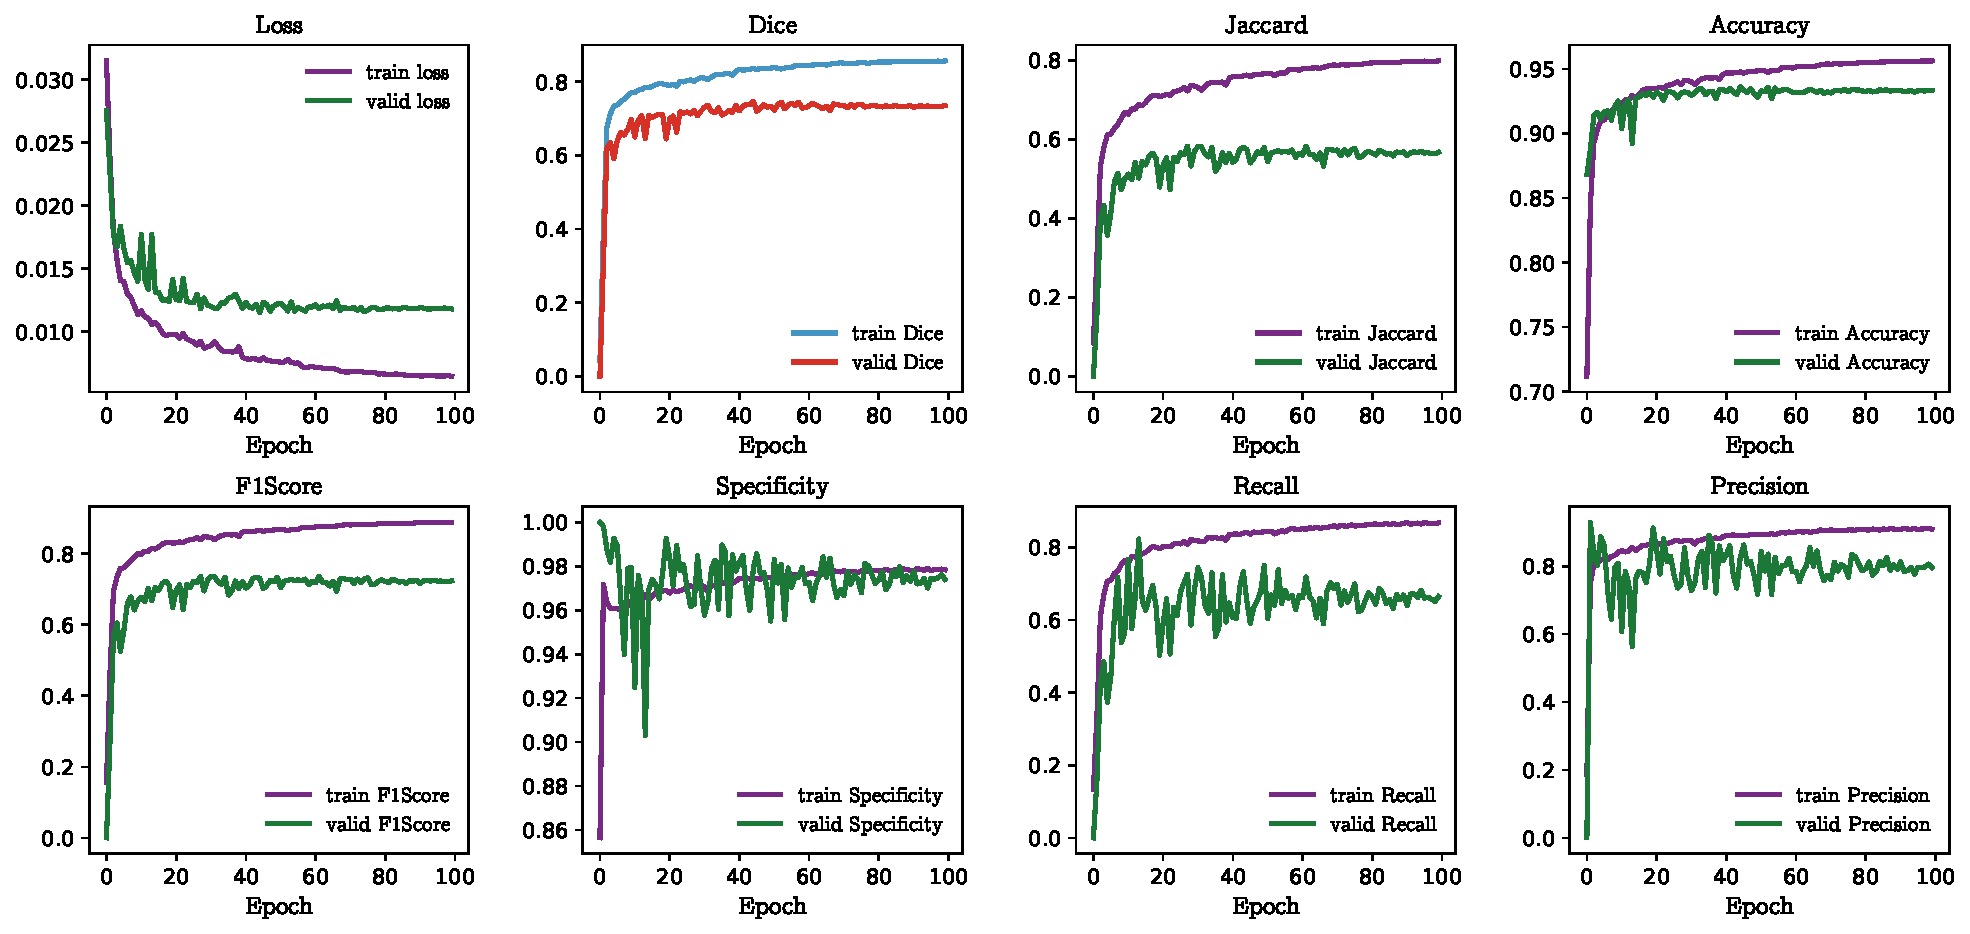
\includegraphics[width=\textwidth]{fig/base_unet_metrics.pdf}
    \caption{基准U-Net模型训练过程中的性能指标变化趋势}
    \label{fig:base_unet_metrics}
\end{figure}

同时,为便于后续实验中基于最优状态进行比较,本研究以验证集 Dice 指标达到最大值的 epoch 作为标准,提取该时刻对应的各项指标结果并作为基准性能对比点,相关数值如表。

\begin{table}[htbp]
    \centering
    \caption{基线U-Net模型在验证集Dice达到最优时(第13轮)的各项性能指标}
    \label{tab:baseline_metrics_horizontal}
    \begin{tabular}{ccccccccc}
        \toprule
        指标 & Dice & F1-score & Jaccard & Precision & Recall & Accuracy & Specificity & Val-Loss \\
        \midrule
        指标值 0.7077 & 0.7030 & 0.5420 & 0.7856 & 0.6266 & 0.9264 & 0.9667 & 0.01312 \\
        \bottomrule
    \end{tabular}
\end{table}

\subsubsection{消融实验结果及分析}


\subsection{泛化性测试}
%在不同医学图像模态(如CT、MRI)和不同器官分割任务中测试改进方法的泛化能力。
%分析模型在不同任务中的表现,验证其在多种场景下的适用性和鲁棒性。


\subsection{方法局限性讨论}
%研究在不同大小的训练数据集下,改进方法的模型性能变化。
%分析模型在小数据集和大数据集上的表现差异,评估其对数据量的敏感性和鲁棒性。

\section{总结与展望}

\subsection{研究工作总结}
%总结本论文的主要研究成果,包括对U - Net网络结构的分析、改进方法的探索以及实验验证的结果。
本文开展的具体研究工作和取得的相应成果主要体现在以下几个方面:

在原有 U-Net 架构的基础上,在跳转连接路径中引入了关注机制。该模块利用编码器提取的高级语义特征来指导低级特征的选择,从而有效抑制可能通过跳转连接传播的背景噪声。实验结果表明,与基线模型相比,利用注意力机制增强的 U-Net 网络在分割性能方面取得了明显的改进。

同时,为了适应不同成像模式的数据集,建立了标准化的数据预处理工作流程,以确保输入数据在训练前保持适当的动态范围。此外,为了增强模型的泛化能力,还采用了几何数据增强技术,如随机图像旋转和水平或垂直翻转。实验结果表明,这些增强策略的应用大大提高了模型缓解过拟合的能力。

本研究还将 DiceLoss 和 CrossEntropyLoss 相结合,构建了一个混合损失函数,同时考虑了区域级轮廓重叠和像素级分类稳定性。这种方法有助于减轻模型训练过程中因分类不平衡造成的负面影响。实验验证证实,使用这种混合损失函数的模型始终优于使用单一损失函数的模型。

最后,本研究通过系统地进行消融和增强实验,有效地整合了有助于提高性能的各种模块和策略,构建了基于 U-Net 的改进模型AAH U-Net。实验结果表明,AAH U-Net 在几乎所有评价指标上的表现都优于其他增强型模型和策略,展示了强大的泛化能力。


\subsection{研究展望}
%对未来进一步研究的方向进行展望,如探索新的网络架构、结合多模态医学图像进行分割等。

以本研究为基础,未来的工作可以围绕三维建模和弱监督学习展开研究:

一方面,目前基于二维切片的处理策略虽然在计算效率上有优势,但难以充分捕捉 CT/MRI 等三维医学影像的层间空间连续性,导致容积分割结果的局部不一致。引入三维卷积或混合维度建模有望通过轴向关注机制或稀疏卷积优化体素级特征融合,在保持解剖结构拓扑完整性的同时提高微小病灶的空间一致性。

另一方面,面对标注成本高昂的临床现实,半监督和自监督学习策略将成为突破数据瓶颈的关键--例如,利用对比学习构建图像表征的先验知识,或通过图像修复、掩膜重建等代理任务挖掘未标注数据的潜在语义信息,可显著降低对全监督信号依赖的依赖,尤其适用于罕见病病理数据或新兴成像模式的快速适应。

最后,还可以深入探索多模态特征融合机制,例如设计一个跨模态注意力模块,通过动态权重分配自适应地整合不同成像模态的判别特征,从而解决单一模态信息缺失或噪声干扰的问题。此外,利用未标记的多模态数据结合对比学习框架对跨模态语义嵌入空间进行预训练,可以显著提高模型在小样本情况下的泛化能力。
\section{总结与展望}

\subsection{研究工作总结}
%总结本论文的主要研究成果,包括对U - Net网络结构的分析、改进方法的探索以及实验验证的结果。

\subsection{研究创新点总结}
%再次强调本研究的创新点及其在医学图像语义分割领域的价值。


\subsection{研究展望}
%对未来进一步研究的方向进行展望,如探索新的网络架构、结合多模态医学图像进行分割等。

%============= 参考文献及附录 ===============
\addcontentsline{toc}{section}{参考文献}
\bibliography{bibfile}

{\zihao{5} \songti \bibliography{bibfile}}     % 设置参考文献的字体为宋体小五号,引用bibfile文件中的文献

%=============  致谢  ======================
\section*{致 ~~ 谢}

行文至此,已是深夜。

首先感谢我的母亲王思敏女士和父亲李正华先生,是你们一路无条件的支持让我走到了今天。
%===================   结束正文    ===============================================================
\end{document}